\section{Introduction}
As discussed in Chapter 1, the attraction effect is a well-studied choice phenomenon where an asymmetrically dominated decoy option increases the choice share of a similar target option \parencite{huberAddingAsymmetricallyDominated1982d}. The attraction effect is an example of a context effect, where choice for an option varies systematically with choice set.

Though context effects originally were originally demonstrated in preferential choice, recent work has generalized these results to simple, perceptual choice. This result has important theoretical and practical implications for decision-making research. I introduce and review this research below.

\subsubsection{From Preferential to Perceptual Choice}

\textcite{choplinComparisoninducedDecoyEffects2005b} and \textcite{yearsleyContextEffectsSimilarity2022} demonstrated the attraction effects in similarity judgments. In both sets of experiments, participants saw various perceptual stimuli (i.e., ovals, swirled lines, vertical lines) and chose the option most similar to a reference option. Both sets of researchers showed that dissimilar decoy options impacted participants' choices as in the attraction Effect

\textcite{trueblood2013not} demonstrated the attraction effect in perceptual choice. In their experiments, participants saw three rectangles on each trial, arranged in a horizontal array, and selected the option they perceived to have the largest area. For an example stimulus set, see Figure~\ref{fig:fig_opts} (right panel). Options $A$ and $B$ have equal area but trade off in height and width. The decoy options ($D_{A}$ and $D_{B}$, respectively) are smaller in area but are more similar to their respective targets than to their respective competitor. In \textcite{trueblood2013not}'s experiments, participants chose the target option more than the competitor option, on average. \footnote{\textcite{trueblood2013not} also demonstrated the similarity and compromise effects.}. 

Notably, the title of \textcite{trueblood2013not}'s paper was "Not Just for Consumers: Context Effects Are Fundamental to Decision Making", and in their General Discussion, \textcite{trueblood2013not} argued "our experiments suggest that these context effects are a general feature of human choice behavior because they are a fundamental part of decision-making processes. As such, our results challenge explanations of these effects exclusively in terms that are unique to high-level decision making and thus call for a common theoretical explanation that applies across paradigms." (p. 907). According to \textcite{trueblood2013not}, context effects are not idiosyncratic to high-level decision-making but are a fundamental feature of choice. \textcite{trueblood2013not} also used these perceptual results to argue against the context-dependent advantage (CDA) model \parencite{tversky1993context} as well as the Leaky Competing Accumulators (LCA) model \parencite{usherLossAversionInhibition2004a}, as these models use loss aversion (the idea that an option's disadvantages on an attribute are weighted more strongly than its advantages on other attributes) to account for context effects (see also \textcite{truebloodPhantomDecoyEffect2017c}). \textcite{truebloodMultialternativeContextEffects2012} demonstrated context effects in an inference task and argued similarly against loss aversion.

\textcite{frederickLimitsAttraction2014b} failed to replicate \textcite{trueblood2013not}'s finding of the attraction effect in perceptual choice. \textcite{frederickLimitsAttraction2014b} collected data online, which may have resulted in less precision than a laboratory task, potentially leading to the null finding.

\textcite{turnerCompetingTheoriesMultialternative2018a} replicated \textcite{trueblood2013not}'s results and performed a large scale modeling analysis, comparing the ability of various model mechanisms to account for context effects. For example, \textcite{turnerCompetingTheoriesMultialternative2018a} concluded that pairwise comparisons on individual attributes greatly improves models' ability to account for context effects. This may not be appropriate, however, given a perceptual domain where dimensions may not be separable \parencite{ashbyVarietiesPerceptualIndependence1986a}. 

\textcite{spektorWhenGoodLooks2018b} followed up on this work and demonstrated the \textit{repulsion effect} in a rectangle choice experiment. In the repulsion effect, the competitor's choice share is higher than the target's choice share \parencite{liaoInfluenceDistanceDecoy2021,evansImpactPresentationOrder2021,simonson2014vices,frederickLimitsAttraction2014b,spektorRepulsionEffectPreferential2022,banerjeeFactorsThatPromote2024,bhui2021rational}. In \textcite{spektorWhenGoodLooks2018b}'s experiments, the target and competitor options varied in area, such that one option was always larger, but on average they were the same size. The researchers also varied the \textit{target-decoy attribute distance} (TDD), the percentage difference between the target and decoy areas. For example, if TDD is $2\%$, the decoy is $2\%$ smaller than the target. 

\begin{figure}
   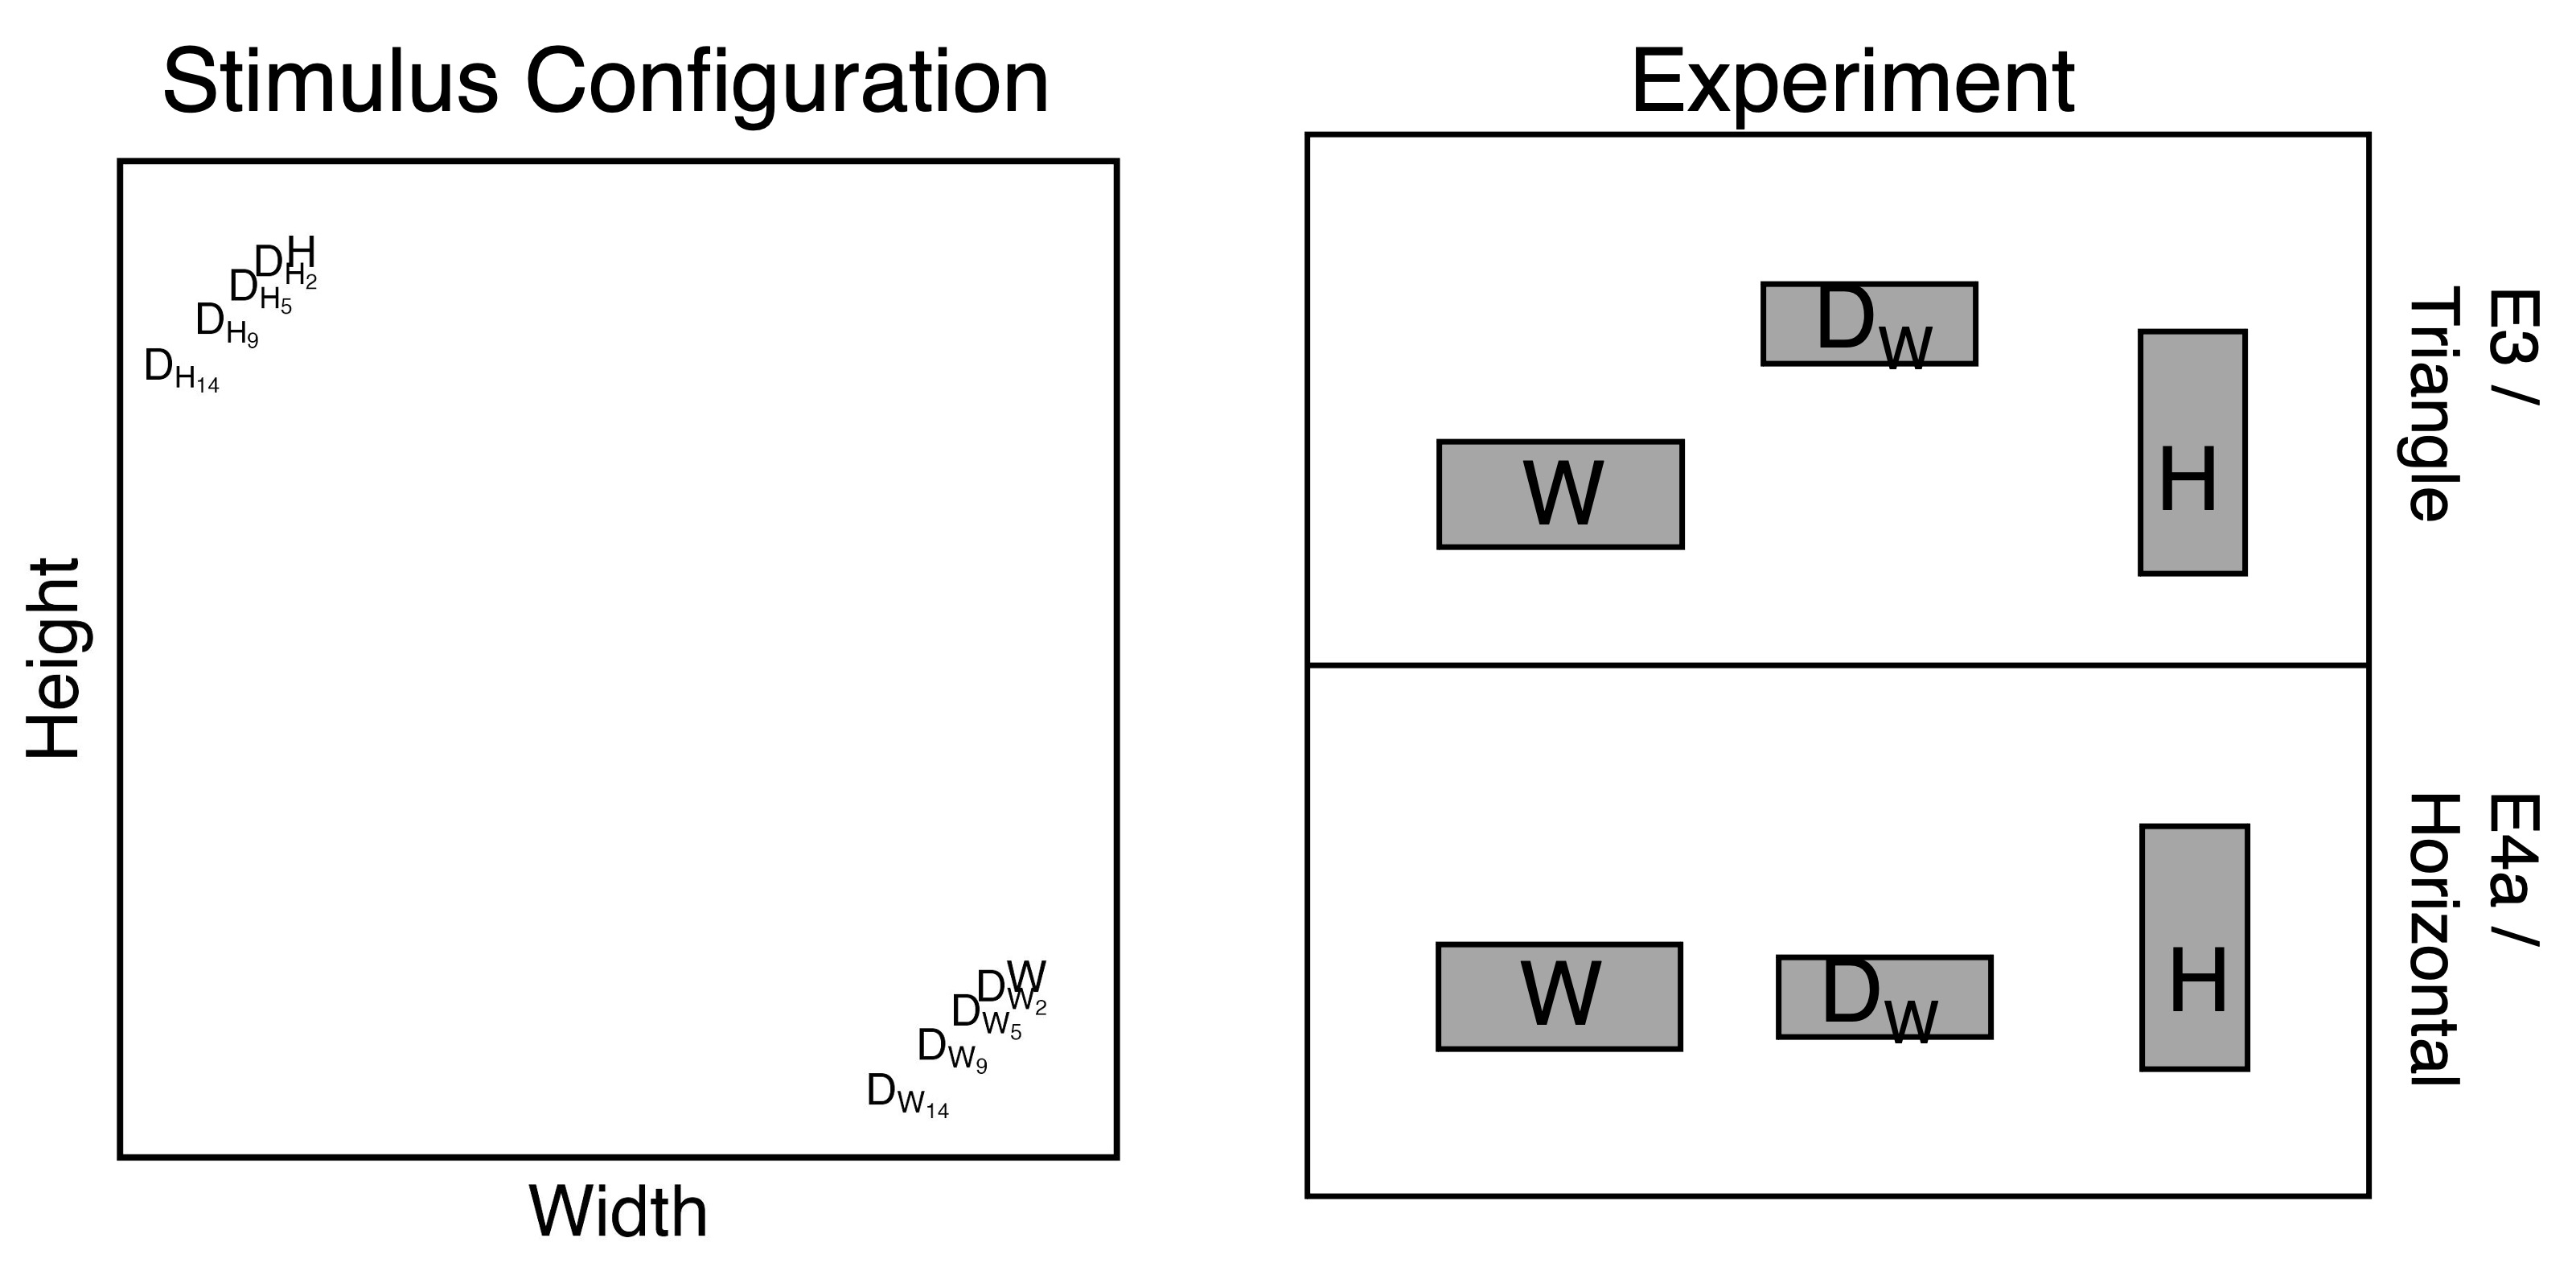
\includegraphics[width=\linewidth]{figures/spektor_stim.png}
   \caption{Stimulus configuration and example trials from \textcite{spektorWhenGoodLooks2018b}, Experiments 3 and 4a. Note that the stimulus in the righthand plot were not shown in the experiment; these are solely for the benefit of the reader.}
   \label{fig:spektor_stim}
\end{figure}

\textcite{spektorWhenGoodLooks2018b} ran a total of five experiments. All experiments showed similar results, so I focus on their experiments 3 and 4a, which are the most representative of the article's conclusions. In Experiment 3, the authors varied TDD at four levels: $2\%$, $5\%$, $9\%$, and $14\%$. The rectangles were arranged in a trianglular display on the screen (see Figure~\ref{fig:spektor_stim}, Experiment 3), in contrast to \textcite{trueblood2013not}'s horizontal display. \textcite{spektorWhenGoodLooks2018b} found an empirical repulsion effect such that the competitor was selected more than the target at all levels of TDD (see Figure~\ref{fig:spektor_data}). 

\textcite{spektorWhenGoodLooks2018b}'s Experiment 4a, however, used the horizontal diplay of \textcite{trueblood2013not} (see Figure~\ref{fig:spektor_stim}, Experiment 4a). Here, they varied TDD at $5\%$, $9\%$, and $14\%$. In Experiment 4a, the data show a slight repulsion effect at low TDD levels that eventually becomes an attraction effect at high TDD levels. 

\textcite{truebloodPhantomDecoyEffect2017c} demonstrated a "phantom decoy" effect in perceptual choice. Phantom decoys are options that are similar to the target, but also superior in value, and are presented but made unavailable at the time of choice. They showed that participants chose the target less than the competitor, i.e., a repulsion effect, a result at odds with phantom decoy effects in preferential choice \parencite{pratkanisBriefHistoryResearch1992b,pettiboneExaminingModelsNondominated2000}. 

\begin{figure}
   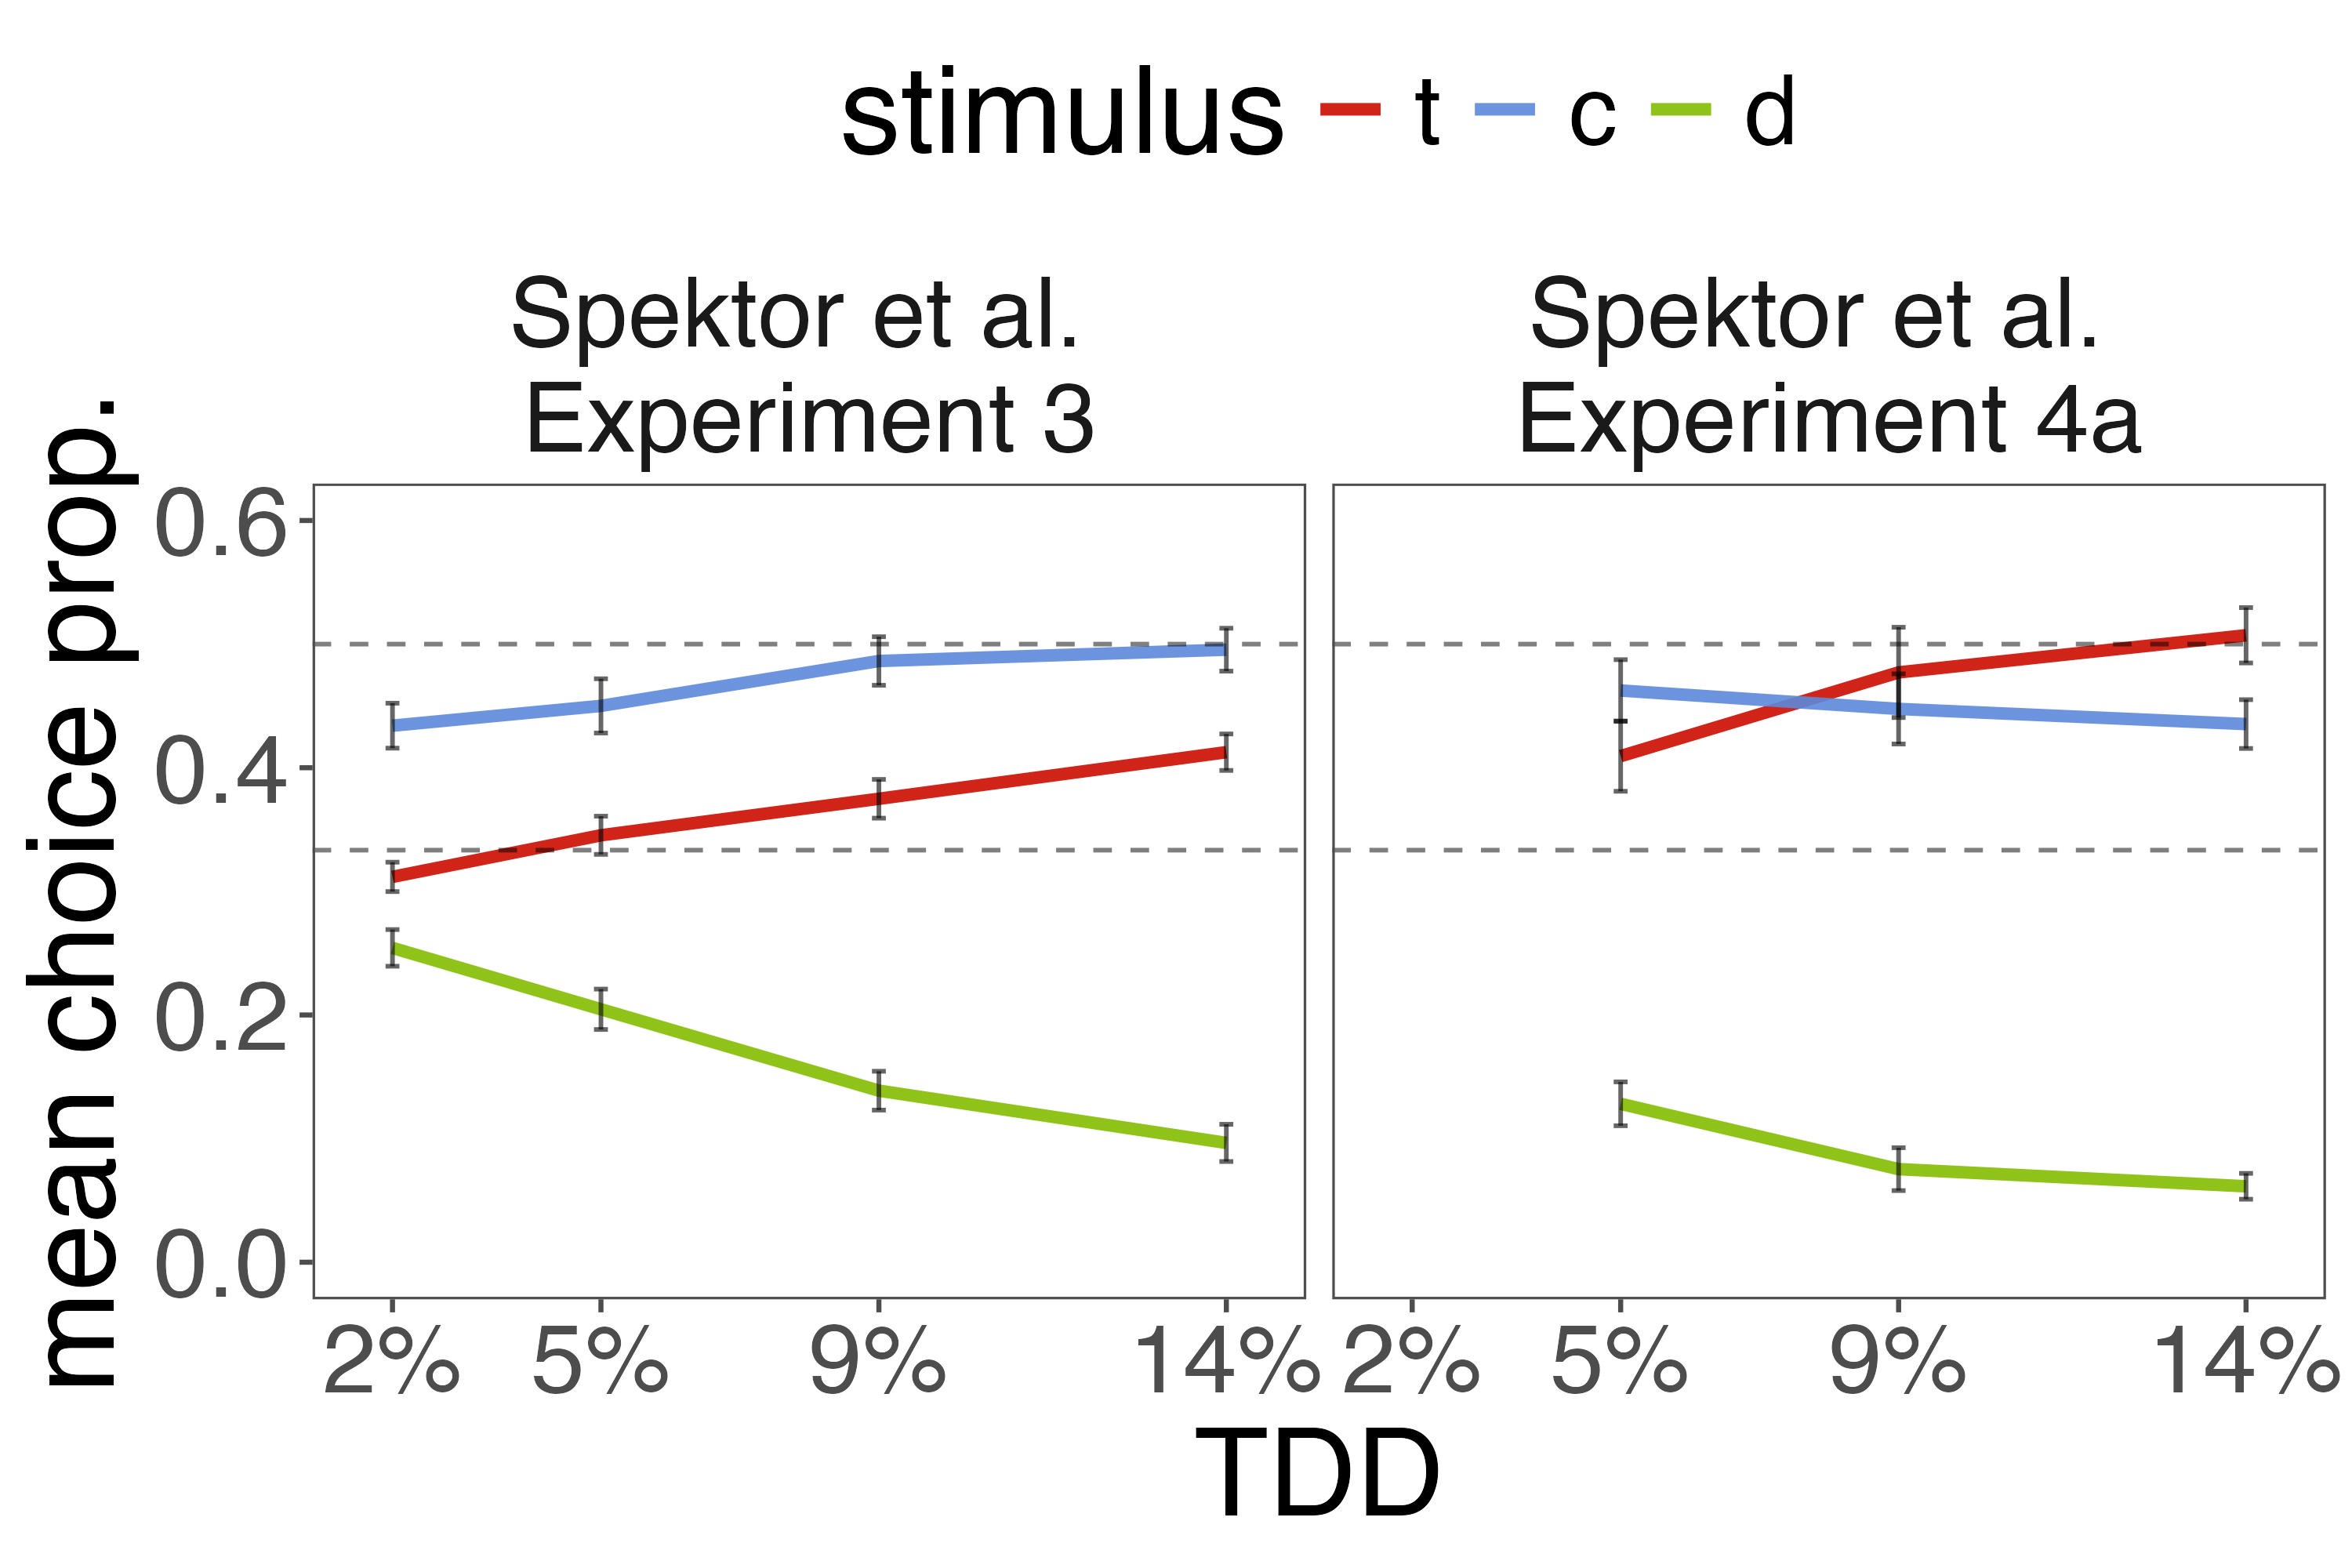
\includegraphics[width=\linewidth]{figures/spektor_data_collapsed.jpeg}
   \caption{Data from \textcite{spektorWhenGoodLooks2018b}, collapsed across choice set. Error bars are $95\%$ CIs of the mean, computed using the within-subjects error correction from \textcite{morey2008confidence}. Dashed lines are drawn at .5 and .33.}
   \label{fig:spektor_data} % might consider graphing (or at least writing RSTs) here
\end{figure}

\textcite{liaoInfluenceDistanceDecoy2021} also replicated the general pattern of \textcite{spektorWhenGoodLooks2018b}'s results and also found a an inverse U-shaped relationship between TDD and the \textit{Relative Share of the Target} RST\footnote{$RST=\frac{P(T|[T,C,D])}{P(T|[T,C,D])+P(C|[T,C,D])}$. $RST>.5$ indicates an attraction effect, while $RST<.5$ indicates a repulsion effect.}. Relatively low and extremely high TDD values created a repulsion effect, while intermediate TDD values created an attraction effect. 

\textcite{spektorRepulsionEffectPreferential2022} demonstrated the repulsion effect in both preferential and perceptual choice, using similar stimuli and a similar display configuration to \textcite{spektorWhenGoodLooks2018b} and \textcite{liaoInfluenceDistanceDecoy2021}. Here, the stimuli were squares containing two bars filled to varying degrees with color. In perceptual choice, participants were to select the stimulus with the largest cumulative filled area. In the preferential choice scenario, participants were told that each filled bar represented one possible outcome of a 50-50 gamble, and they were to select the gamble with the highest expected value. Their results were similar to those of \textcite{spektorWhenGoodLooks2018b}, however, where target and competitor choices increased with TDD.

Researchers are clearly using perceptual experiments to demonstrate context effects and test theory. These results are clearly informative and theoretically interesting. I argue, however, that researchers should be cautious in assuming that decision-makers receive perceptual input with the same accuracy that they do in preferential choice experiments. Researchers should seek to separate the role of perceptual discriminability from decisional processes when understanding participants' responses. I elaborate on these ideas below and in Chapter 2, with a demonstration using the results of \textcite{spektorWhenGoodLooks2018b}.

\subsection{Understanding Perceptual Choice Experiments}

A crucial assumption made by researchers in the above experiments, is that the perceptual difficulty of these tasks does not affect the conclusions. Researchers often assume that the chocie data in perceptual choice experiments can be analyzed identically to that of preferential choice experiments. Participants regularly fail to perceive that the decoy is the smallest stimulus in the choice set, and this discriminability failure affects target choices more than competitor choices. Researchers tend to assume that, to the extent that the dominance relationship is misperceived, the decoy is equally likely to be seen as larger than the target than larger than the competitor. 

One plausible account of \textcite{spektorWhenGoodLooks2018b}'s data is that participants occasionally misperceive the dominance relationship, and due to the difficulty of the task and the similarity of target and decoy, are more likely to choose the decoy over the target than the competitor. Such a process creates an empirical repulsion effect but is qualitatively different than a reversal of the traditional attraction effect. \textcite{spektorWhenGoodLooks2018b} dismiss such an account because the target is chosen more often the decoy; however, this fact does not rule out the above explanation of the data.

One goal of this dissertation is to separate the role of perceptual and decisonal processes in context effects. To do so, I begin with an extreme stance - that such experiments are solely perceptual experiments rather than decision-making experiments and that no high level decision processes are occurring. This extreme assumption is likely incorrect, but it may be helpful in understanding existing data. To begin, I return the results of \textcite{spektorWhenGoodLooks2018b}. 

As reported above, \textcite{spektorWhenGoodLooks2018b} demonstrate that a relatively small change in stimulus display (arranging stimuli in a triangle rather than a horizontal line) reverses the attraction effect. Why is it that a relatively subtle change in stimulus display led to a qualitative shift in the data? To answer this question, I highlight the differences between \textcite{spektorWhenGoodLooks2018b}'s data and previous context effect experiments. 

In preferential choice tasks, participants are given a set of options on each trial (e.g., laptops, apartments, washing machines), along with the attribute values associated with each option (e.g., 10 GB RAM, 1500 square feet, 2.7 cubic feet capacity). These attributes are typically represented numerically \parencite{hayes2024attribute,banerjeeFactorsThatPromote2024} or with easily discriminable graphical representations \parencite{cataldoComparisonProcessAccount2019b}. The decoy option, therefore, is rarely selected (e.g., $<5\%$ of all trials in many studies), and these selections are assumed to be the result of inattention or accidental responses. Researchers can reliably assume that participants are able to detect the dominance relationship between target and decoy. Perceptual choice tasks complicate participants' ability to detect this dominance relationship. 

In \textcite{spektorWhenGoodLooks2018b}'s experiments, the decoy is selected as often as $25\%$ of all trials in some conditions. The decoy is selected less often in experiment 4a (triangle display) than in experiment 3 (horizontal display). Decoy selections also decrease as the difference between decoy area and target/competitor areas increases. Finally, though both target and competitor increase in choice share as TDD increases, the target choice share increases at a higher rate than does the competitor, suggesting a strong trade-off between target and decoy choices; stronger, indeed, than the competitor-decoy trade-off. That is, the mean \textit{Relative Share of the Target} (RST) \parencite{berkowitschRigorouslyTestingMultialternative2014b} increases with TDD in both experiments 

Clearly, perceptual discriminability plays a role in \textcite{spektorWhenGoodLooks2018b}'s results. Participants clearly are better able to discriminate the target and competitor from the decoy as the decoy decreases in size. Any reasonable account of these data should parse the out discriminability from genuine context effects. To do so, I turn to a well-studied class of models within the psychology literature.

\subsection{Modeling Context-Dependent Perceptual Choice}

There is a large body of psychological research, beginning with the work of \textcite{thurstone1927law}, of treating the perception of a stimulus as a random variable. In his famous "Law of Comparative Judgment" paper, \textcite{thurstone1927law} first showed that researchers can use binary choice proportions to estimate the psychological distance between stimuli, by treating perceptual intensity as a Gaussian random variable. Models of this class are often called \textit{Thurstonian}, a term I use throughout this dissertation. 

Thurstone's work led to similar research using Signal Detection Theory (SDT) \parencite{hautus2021detection}, which also treats psychological quantities (e.g., memory, perception), as random variables. Similarly, Ashby and colleagues' General Recognition Theory (GRT) models the perception of a single stimulus as a multivariate normal random variable, where each dimension of the model is the perceived dimension of a stimulus \parencite{ashbyVarietiesPerceptualIndependence1986a,ashby1988decision, ashbyUnifiedTheorySimilarity,maddoxComparingDecisionBound1993}. In marketing and economics, researchers treat the utilities of choice options as random variables, which are often assumed to be Gaussian or Extreme Value Distributed and estimate choice models known as Random Utility Model (RUMs) \parencite{mcfadden2001economic,hausman1978conditional,train2009discrete}. Often, though not necessarily, these models share the common property that value - be it the utility of a consumer product, the perception of magnitude in a perceptual task, or memory signal in a recognition task - is stochastic while choice is deterministic  (c.f. \textcite{benjamin2009signal}).

Based on this large body of research, I now introduce the Thurstonian model I explore throughout the dissertation. This model is simplistic, as it treats the experiments of \textcite{trueblood2013not} and \textcite{spektorWhenGoodLooks2018b} as perceptual, rather than decision tasks. This also completely eschews the possibility of higher level decision processes. I use this model to differentiate perceptual from decision-making processes in the repulsion and attraction effects. The model treats value (perceived area) as stochastic and choice as deterministic. Furthermore, I do not treat height and width as independent attributes but rather consider perceived area to be unidimensional. 

I assume that on each trial $i$ with choice set $K$, the perception $\mathbf{X_i}$ of all $3$ stimuli is sampled from a multivariate Gaussian distribution with a mean vector $\boldsymbol{\mu}$ and variance-covariance matrix $\boldsymbol{\Sigma}$:

\begin{align}
   \mathbf{X}_{i} \sim \mathcal{N}(\boldsymbol{\mu}, \boldsymbol{\Sigma})
   \label{eqn:mvnorm}
\end{align}

where $\boldsymbol{\mu}$ is the column vector:
\begin{align}
   \begin{pmatrix}
      \mu_{T} \\
      \mu_{C} \\
      \mu_{D}
      \end{pmatrix}
   \label{eqn:mu}
\end{align}

where the subscripts $T$, $C$, and $D$ indicate target, decoy, and competitor, respectively, and $\boldsymbol{\Sigma}$ is a positive semi-definite $3 \text{x} 3$ covariance matrix computed as:

\begin{align}
   \boldsymbol{\Sigma}=S\boldsymbol{\Omega}S
   \label{eqn:Sigma}
\end{align}

where $S$ is a diagonal matrix consisting of: 

\begin{align}
   \begin{pmatrix}
      \sigma_{T} & 0 & 0 \\
      0 & \sigma_{C} & 0 \\
      0 & 0 & \sigma_{D} 
   \end{pmatrix}
\label{eqn:S}
\end{align}

with $\sigma_{T}$, $\sigma_{C}$, $\sigma_{D}$ being the standard deviations for target, competitor, and decoy, respectively. $\boldsymbol{\Omega}$ is a correlation matrix:

\begin{align}
   \begin{pmatrix}
      1 & \rho_{TC} & \rho_{TD} \\
      \rho_{TC} & 1 & \rho_{CD} \\
      \rho_{TD} & \rho_{CD} & 1 
   \end{pmatrix}
\label{eqn:O}
\end{align}
with $\rho_{TD}$, for example, indicating the population-level correlation between target and decoy perecptions.

As mentioned above, the model assumes that value is stochastic while choice is deterministic\footnote{This also assumes ties are not possible, which is true if and only if perceived area is absolutely continuous.}. The model always chooses the option perceived as largest, regardless of the magnitude of the difference between the "winner" and "runners-up". That is, given a vector $\mathbf{X}_i$ of perceived areas on trial $i$ with set $K$, the probability a participant selects stimulus $j$ is:

\begin{align}
   P(j|i,K)=P(\mathbf{X}_{ij}>\mathbf{X}_{ik}), \forall k \in K, j \neq k
   \label{eqn:pchoice}
\end{align}

If all off-diagonal elements of $\boldsymbol{\Omega}$ are $0$ and $\sigma_{T}=\sigma_{C}=\sigma_{D}$, the model collapses to the standard Thurstonian Case V model \parencite{thurstone1927law} often used by cognitive psychology researchers. Models of this form have closed form solutions and their predictions are easy to compute.

On the other hand, if any elements of $\boldsymbol{\Omega}$ are non-zero, the closed form solution of this model does not exist, and to compute predictions and estimate model parameters, researchers must use simulation or numerical integration methods \parencite{train2009discrete}. In all applications of these model through this dissertation, I use simulation to generate model predictions. 

This model is capable of generating a(n) attraction (repulsion) effect by assuming $\mu_{T}>\mu_{C}$ ($\mu_{C}>\mu_{T}$), i.e., that on average target and competitor stimuli differ in their perceived areas. This, however, is an ad hoc assumption that may describe the data well but will generate limited theoretical insight. Moreover, I wil later present empirical data that suggest, generally speaking, $\mu_{T}\approx\mu_{C}$. 

I used model simulations to assess the effect of correlations (.e., $\rho_{TC}$, $\rho_{TD}$, and $\rho_{CD}$) on predictions for the attraction and repulsion effects. 

I varied both $\rho_{TD}$ and $\rho_{TC}$ from -1 to 1; in other words, all rectangles oriented the same way share one correlation and those oriented differently share another correlation. I show model predictions that result from varying these correlations in Figure~\ref{fig:3d_model}. Here, I assume that $\mu_{T}=\mu_{C}>\mu_{D}$ and that $\sigma_{T}=\sigma_{C}=\sigma_{D}$\footnote{In Experiment 2 I present evidence supporting these assumptions.}. 

Figure~\ref{fig:3d_model} shows model predictions in the form of $RST$ (Relative Share of the Target), where RST values above .5 indicate an attraction effect and values below .5 indicate a repulsion effect. The model can, depending on the relationship between $\rho_{TD}$ and $\rho_{TC}$, predict a repulsion, attraction, or a null context effect. If $\rho_{TD}>\rho_{TC}$, the model predicts a repulsion effect. If the target and decoy are correlated more strongly than competitor and decoy, it is more likely that if on a particular trial the target perception is large, that the decoy is even \textit{larger}, causing the decoy to "steal" choice shares from the target more than the competitor, i.e., a repulsion effect.

\begin{figure}
   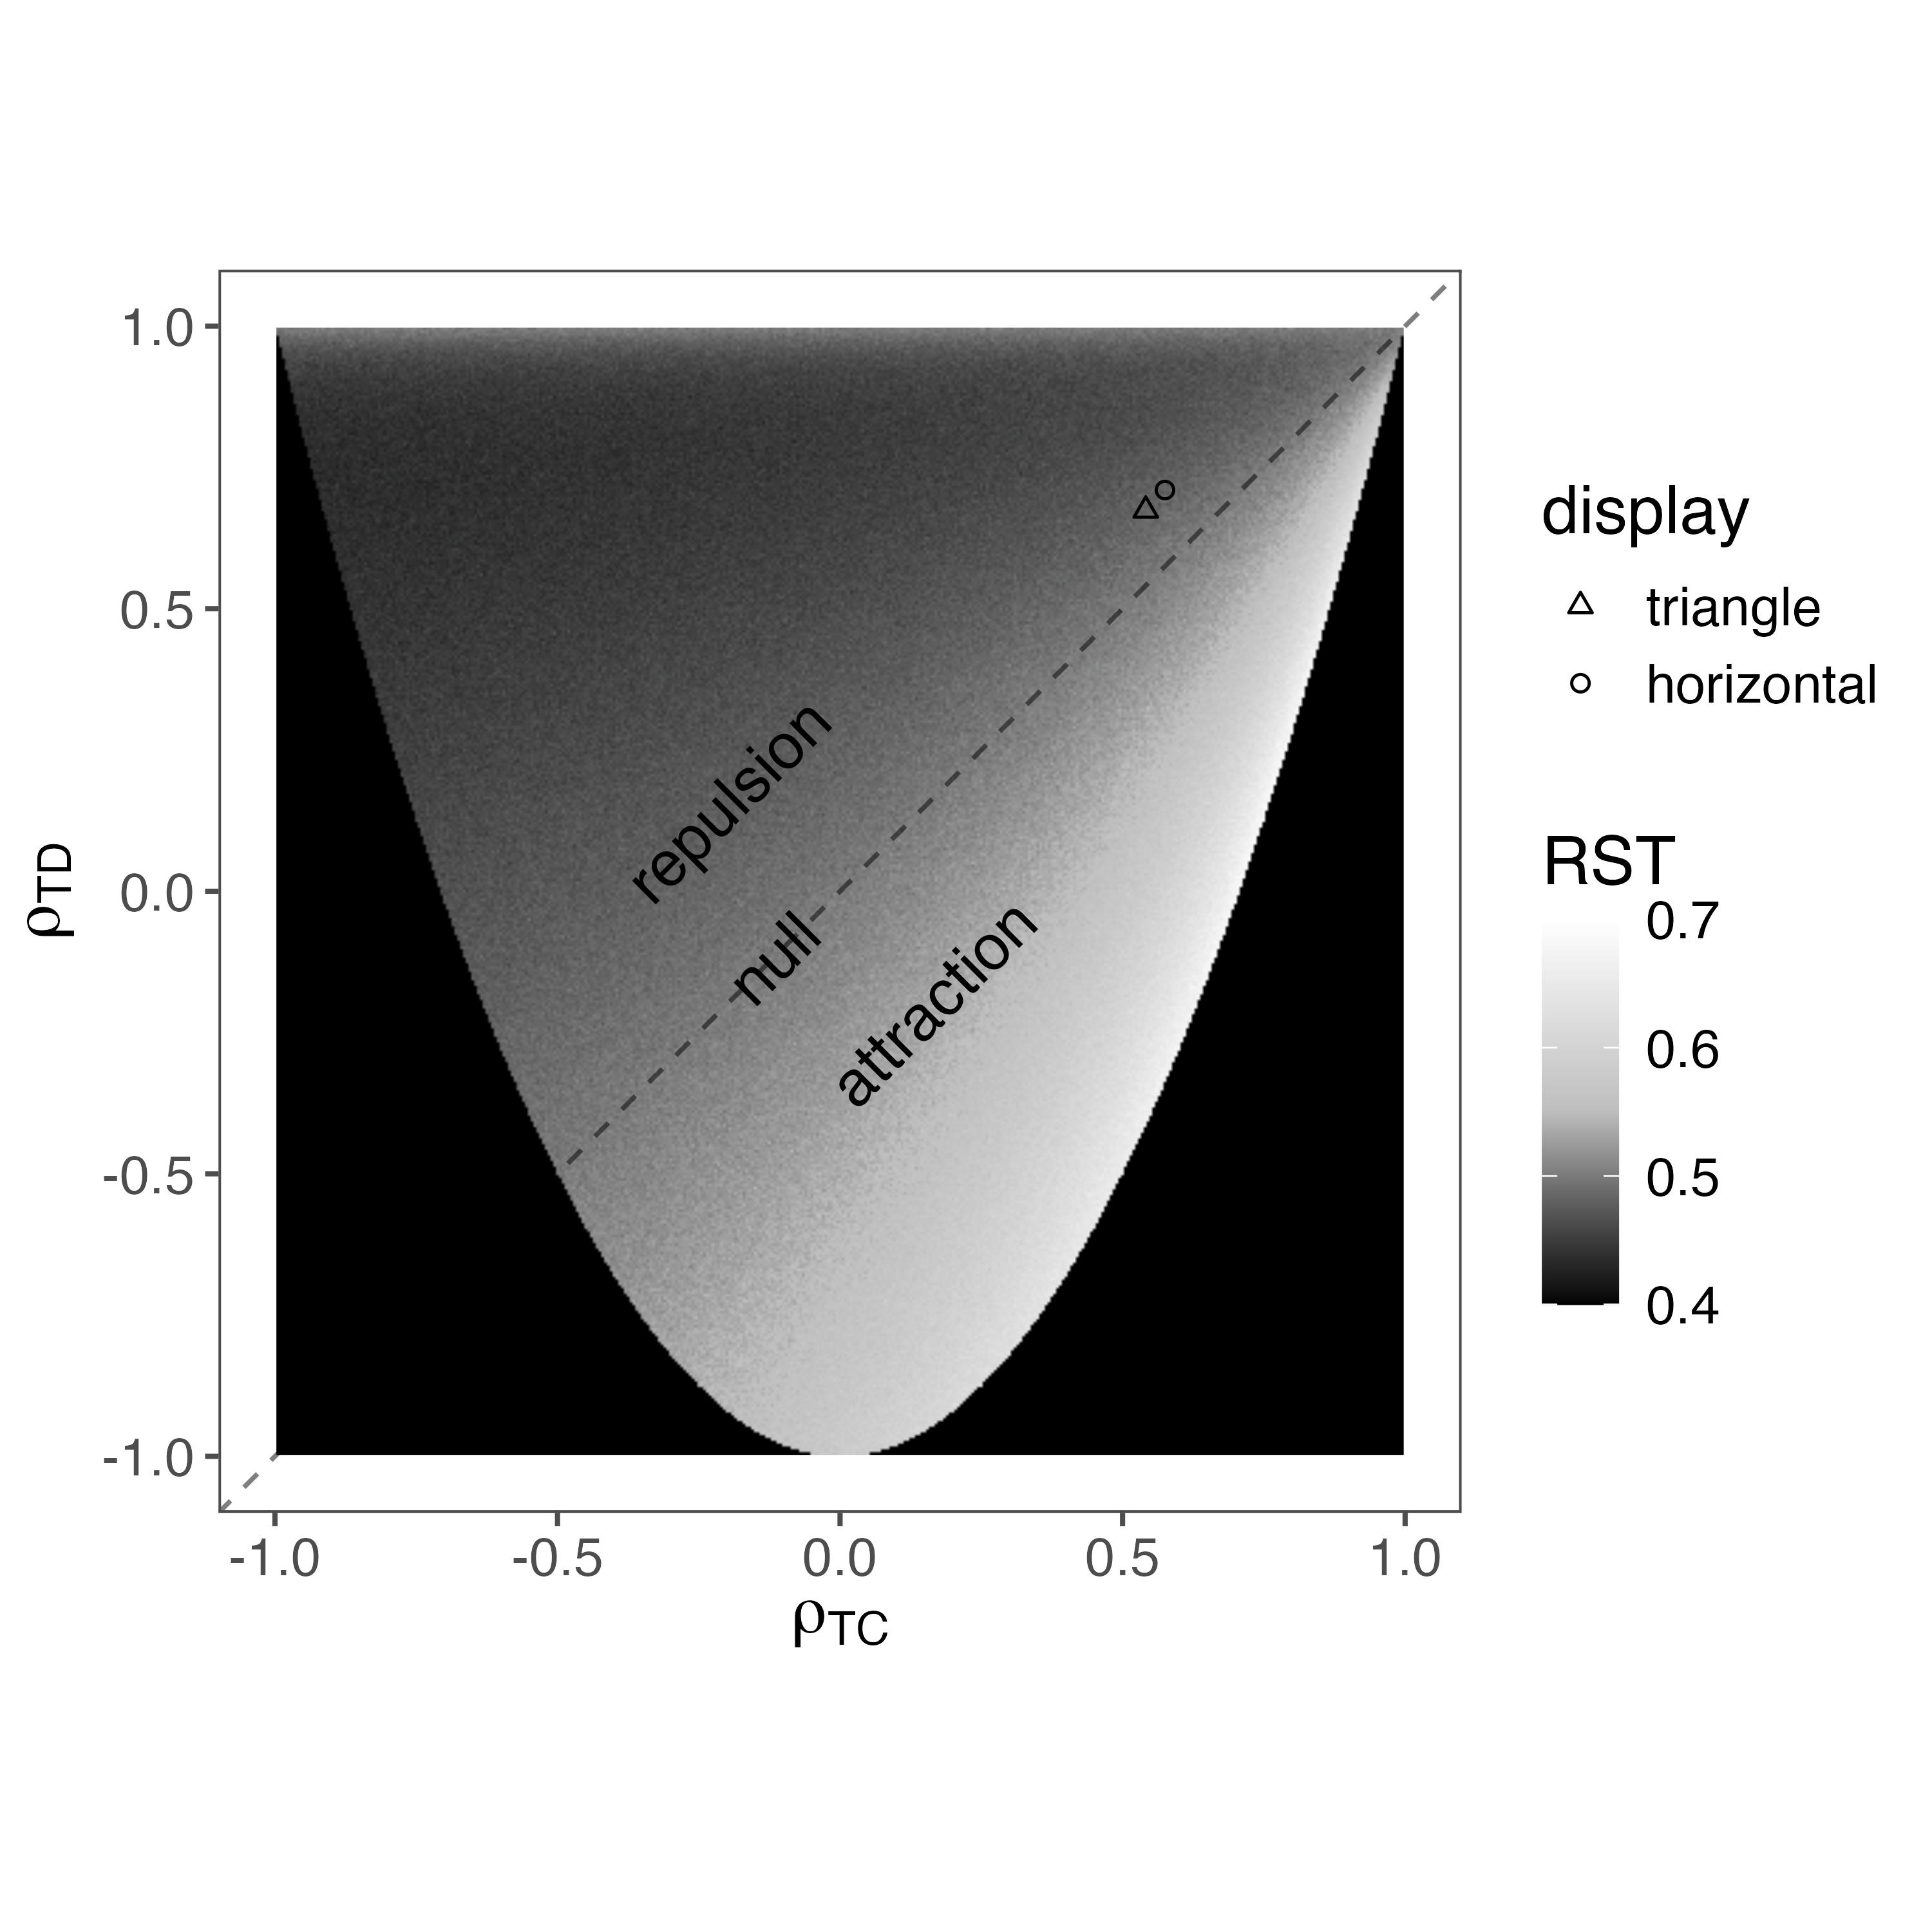
\includegraphics[width=\linewidth]{figures/3d_sim_rst.jpg}
   \caption{Model simulations for the attraction and repulsion effects based on the variation of $\rho_{TD}$ and $\rho_{TC}$. "Regions" of the plot are labeled based on their qualitative predictions for attraction, null, and repulsion effects. The black region is the area where, due to extreme correlations, a positive semi-definite variance-covariance matrix could not be formed and predictions are unavailable. The triangle and circle mark the estimated mean correlations from the Experiment 2 triangle and horizontal conditions, respectively.}
   \label{fig:3d_model}
\end{figure}

If $\rho_{TD}<\rho_{TC}$, the model predicts an attraction effect. This is because $\rho_{TC}=\rho_{CD}>\rho_{TD}$, so the decoy "steals" choice shares from the competitor more than the target.

Finally, if $\rho_{TD}=\rho_{TC}=\rho_{CD}$, the model predicts a null effect. In this case, no pair of stimuli are more correlated than any other pair, so the predictions are identical to a model where $\rho_{TD}=\rho_{TC}=\rho_{CD}=0$ model. 

\subsection{Perceptual Correlations as Mechanism for the Repulsion Effect}
I propose that these perceptual correlations may be driving the repulsion effect in \textcite{spektorWhenGoodLooks2018b}'s data. The decoy option is smaller than the the target and competitor options and is thus not always discriminated. The triangle configuration makes discriminability particularly difficult for participants (as I show below in Experiment 1). Simultaneously, however, the fact that target and decoy share an orientation (i.e., both wide or both tall) makes the comparison of these two options easier. When TDD is low, the ease of target-decoy comparison will increase the likelihood that the decoy is perceived to be larger than the target. In statistical terms, the perception of the decoy is more strongly correlated with the perception of the target than with perception of the competitor. These correlations are measured with the $\rho_{TD}$ and $\rho_{CD}$ parameters. According to this account, if $\rho_{TD}>\rho_{CD}$, the perceived areas of target and decoy "move" together, allowing the competitor to exceed the target at a higher rate than the target exceeds the competitor, particularly if perceptual discriminability is low. The repulsion effect may thus be driven by perception rather than decision processes. 

In Experiment 1, I first present results from a two-alternative forced-choice experiment to show that these stimuli are easily confusable and that the triangle display of \textcite{spektorWhenGoodLooks2018b} decreases discriminability relative to the horizontal display. I also show that, consistent with the predictions of a Thurstonian perceptual model where $\rho_{TD}>\rho_{TC}=\rho_{CD}$, target-decoy discriminability is in fact greater than competitor-decoy discriminability in binary choice and that target-decoy discriminability increases with TDD. 

\section{Experiment 1}

The goal of Experiment 1 was to test participants' ability to discriminate between rectangles in the perceptual choice tasks of \textcite{trueblood2013not} and \textcite{spektorWhenGoodLooks2018b}. 
On each trial, participants saw three options (target, competitor, and decoy). After a short delay, two of the rectangles were highlighted and participants chose which of the two rectangles was larger. 
This experiment also included a within-subjects manipulation to compare discriminability in both the triangle display of \textcite{spektorWhenGoodLooks2018b}, Experiment 3, and the horizontal display of \textcite{spektorWhenGoodLooks2018b}, Experiment 4a\footnote{see also \textcite{trueblood2013not}, Experiment 1.}. Otherwise, with a few exceptions discussed below, I follow the stimulus construction and experimental design of \textcite{spektorWhenGoodLooks2018b}, Experiments 3 and 4a. 

\subsection{Methods}

\subsubsection{Participants.}
Data collection took place at the University of Massachusetts Amherst. 86 undergraduate students participated in exchange for course credit. 1 participant who achieved less than $80\%$ accuracy on catch trials (see below) was excluded from all analyses. Trials with response times (RTs) $<100\text{ms}$ or  $>10000\text{ms}$ were also excluded from all analyses.

\subsubsection{Stimuli.}
The experiment had two types of trials: critical trials and catch trials. 
On each critical trial, the target and competitor had the same area\footnote{Here I simplify \textcite{spektorWhenGoodLooks2018b}'s design by ensuring both focal stimuli had the same area.} but differed on orientation, with one stimulus being wide and the other tall. The decoy always had the same orientation as the target. The height and width of the decoy were reduced proportionally so that the decoy area was always $0\%$, $2\%$, $5\%$, $9\%$, or $14\%$ of the target areas. Because the target and competitor always had the same area, this means that the decoy was also $0\%$, $2\%$, $5\%$, $9\%$, or $14\%$ of the competitor area. These are the TDD values from \textcite{spektorWhenGoodLooks2018b}, plus a $0\%$ level which acted as a baseline\footnote{When TDD=$0\%$, the target and decoy are identical, so labeling is arbitrary.}.

\subsubsection{Design.}
There were 5 blocks of trials. In each block there were 60 critical trials, 12 at each TDD level, and 30 catch trials. Of the 12 critical trials at each TDD level, 6 were presented in a triangle and 6 were presented horizontally.. Finally, 3 of the 6 targets in each display condition at each TDD level were wide and 3 were tall. Of each of these 3, one was a target-decoy comparison, one was a target-competitor comparison, and one was a competitor-decoy comparison. Trial order and rectangle order within each trial were randomized. Thus, this was a $4$ (TDD: $2\%$, $5\%$, $9\%$, $14\%$) x $2$ (display: triangle, horizontal) x $2$ (target-decoy orientation: wide, tall) x $3$ (comparison: target-decoy, target-competitor, competitor-decoy) within-participants design. 

On each catch trial, there was one large rectangle and two much smaller rectangles. The large rectangle was $260 \pm U(-40, 40) \text{x} 200 \pm U(-40, 40)$ pixels, with a random orientation. The smaller rectangles were $180 \pm U(-40, 40) \text{x} 120 \pm U(-40, 40)$ pixels, one wide and one tall.

On every trial, the rectangles were displayed in either a triangle or horizontal display (see Figure~\ref{fig:spektor_stim}). The horizontal distance between all rectangles was constant, but 25 pixels of jitter was added to each rectangle's vertical location.

Stimuli were presented on computer monitors with a resolution of 1920 x 1080 pixels. The experiment was programmed with jsPsych \parencite{deleeuwJsPsychJavaScriptLibrary2015}. 

\subsubsection{Procedure.}
On each trial, participants saw three rectangles, labeled 1, 2, and 3 (from left to right). The rectangles appeared for $1825ms$ total, but after $500ms$, two of the rectangles changed to a darker shade. After all three rectangles disappeared from the screen, participants were asked to select which of the two darker rectangles had the larger area.

\subsection{Results}

\subsubsection{Catch Trials.}
Participants performed well on the catch trials. The mean percentage correct in the triangle display was $92.6\% (SD=3.77)$, and the mean percentage correct in the triangle display was $93.2\% (SD=3.52)$. 

\subsubsection{Critical Trials.}
I first checked the baseline TDD level data (TDD=$0\%$) across to make sure that participants were indifferent between pairs of options when they had identical area. The mean percentage of target choices in target-competitor trials was $48.99\%$ (SD=10.18). The mean percentage of competitor choices in competitor-decoy trials was $49.80\%$ (SD=11.30). The mean percentage of target choices in target-decoy trials was $49.47\%$ (SD=12.06). Participants were indifferent between all pairs of options in the $\text{TDD}=0\%$ trials, so I do not consider these trials further.

The primary analysis was performed on the target-decoy and competitor-decoy trials, excluding the TDD=$0\%$ trials. In these trials participants' task is simply to not select the decoy option on a given trial. I present mean choice proportions across conditions in Figure~\ref{fig:e1_data}. Participants' performance indeed improves with TDD. Furthermore, their performance is better when stimuli are displayed in the horizontal configuration than in the triangle configuration, and it is also better in target-decoy trials compared to competitor-decoy trials. Finally, there is an interaction, such that as TDD increases, the target-decoy performance is even better than the competitor-decoy performance. See the Appendix for inferential statistics which support these conclusions.

\begin{figure}
   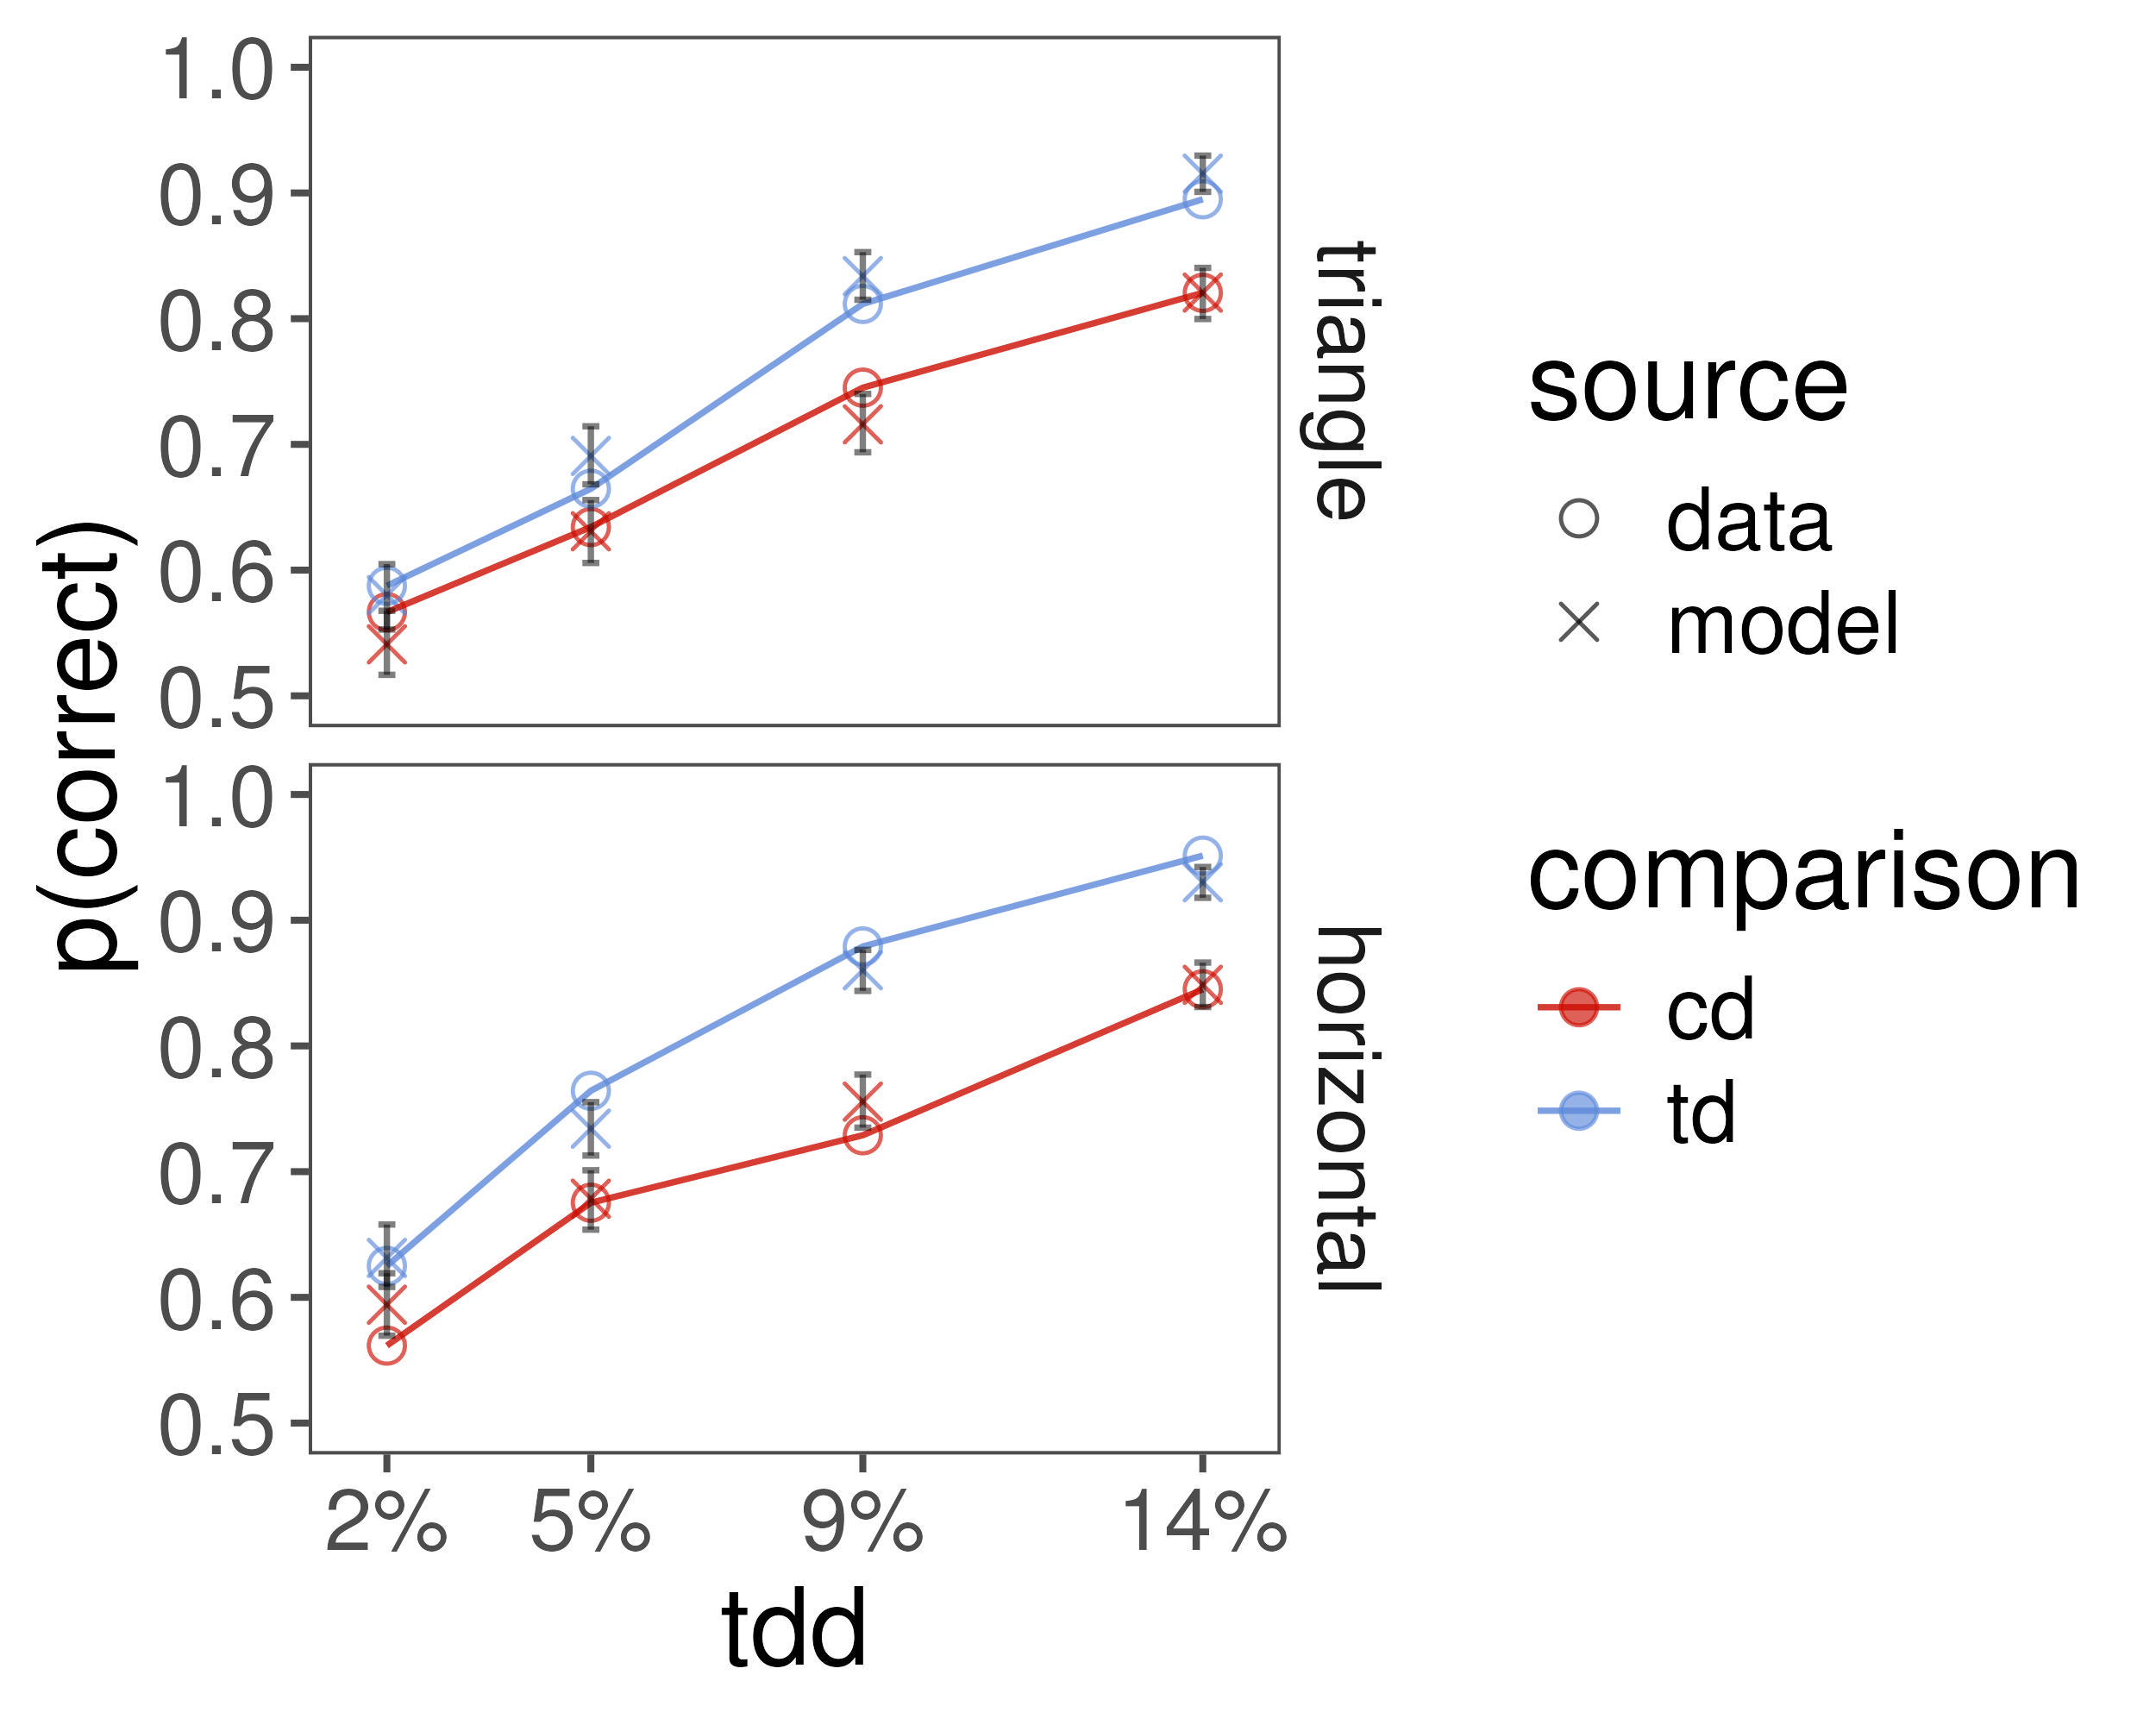
\includegraphics[width=\textwidth]{figures/m14_model_preds_v_data.jpeg}
   \caption{Experiment 1, mean choice proportions by stimulus display, TDD, and comparison. td=target-decoy trials, cd=competitor-decoy trials. Model predictions come from the Bayesian hierarchical logistic regression presented in the Appendix. Error bars are $95\%$ HDIs on the mean.}
   \label{fig:e1_data}
\end{figure}

\subsubsection{Discussion}
In Experiment 1, I showed that participants are not always able to discriminate between target-decoy and competitor-decoy stimuli. I also show that this discriminability increases with TDD and that overall discriminability is better in the horizontal compared to the triangle display. Finally, through the interaction of comparison-pair and TDD, I show that target-decoy discriminability increases with TDD at a higher rate than competitor-decoy discriminability. 

It may seem counterintuitive that target-decoy correlations can simultaneously create greater 2afc discriminability. To understand this, it may help to express the correlation $\rho_{TD}$ as:

\begin{equation}
   \rho_{TD}=\frac{\mathbb{E}[(X_{T}-\mu_{T})(X_{D}-\mu_{D})]}{\sigma_{T}\sigma_{D}}
   \label{eqn:rho_expectation}
\end{equation}

As $\rho_{TD}$ increases, the difference between sampled target and decoy values converges towards the true difference between $\mu{T}$ and $\mu_{D}$. I also show this by plotting the difference in sampled target and decoy values against increasing values of $\rho_{TD}$.

\begin{figure}
   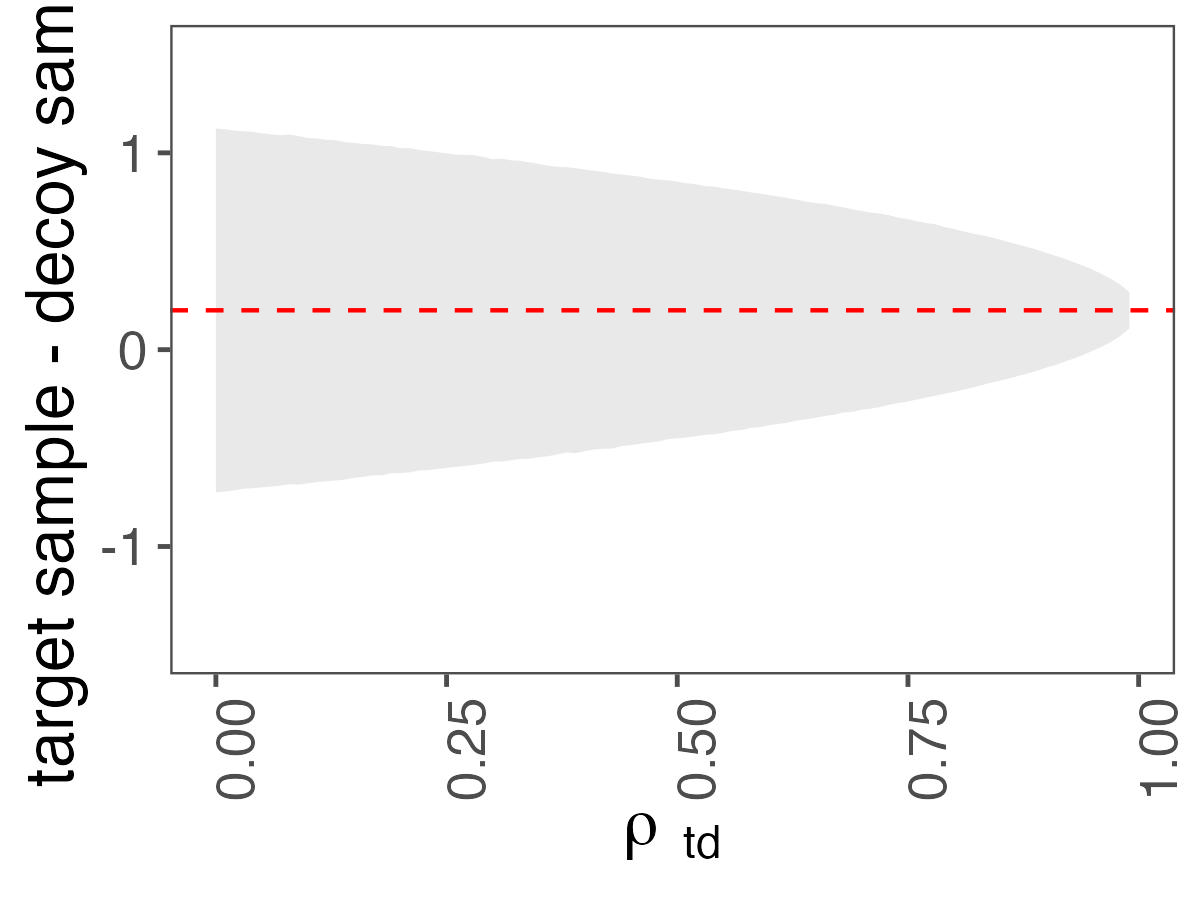
\includegraphics[width=125mm]{figures/sim_mvnorm_vary_r_td.jpeg}
   \caption{Simulated differences in sampled target minus decoy area (i.e., $X_{T}-X_{D}$) as an plotted against increasing values of $\rho_{TD}$. The lower and upper boundaries of the polygon show the lower and upper quantiles of the difference ($2.5\%$ and $97.5\%$), respectively.}
   \label{fig:sim_mvnorm_vary_r_td}
\end{figure}

These results are important because they show that target-decoy (and indeed, competitor-decoy) discriminability cannot be taken as a given in perceptual context effect experiments. Researchers must carefully consider how perception of the decoy affects choice. This is important theoretically because any conclusions about context effects being fundamental to choice \parencite{trueblood2013not} rely on the assumption that context effects are qualitatively similar across choice domains.

In Experiment 2, I combined a psychophysics task with a choice task to estimate the parameters of the Thurstonian perceptual model outlined in the beginning of this chapter. In the first phase of the experiment, participants estimate the size of target, decoy, and competitor rectangles on each trial. In the second phase of the experiment, I conducted a standard choice experiment, replicating \textcite{spektorWhenGoodLooks2018b}'s results. I used the data from the first phase of Experiment 2 to obtain stable estimates of  $\boldsymbol{\mu}$ and $\boldsymbol{\Sigma}$ in the Thurstonian perceptual model. Finally, I show that the model, conditioned on the current parameter estimates, naturally predicts a repulsion effect but not an attraction effect.  

\section{Experiment 2}
The goal of this experiment was to estimate the parameters of the model presented above and to clarify the role of perception and decision in producing the repulsion and attraction effects. I used the \textit{method of cross-modal matching} \parencite{stevensCrossmodalityMatchingBrightness1965} to do so. 

In Experiment 2, participants adjusted the size of a circle to match the perceived area for each rectangle. On each trial, participants saw three rectangles and three circles, each labeled 1, 2, and 3. Participants adjusted the size of the circle corresponding to each rectangle, until they believed the two to have equal area. I also replicated \textcite{spektorWhenGoodLooks2018b}'s choice data in the second phase of the experiment. In both phases, I used a between-subjects manipulation to display the rectangle stimuli in either the horizontal or triangle displays of \textcite{spektorWhenGoodLooks2018b}.

\subsection{Methods}
\subsubsection{Participants.}
Data collection took place at the University of Massachusetts Amherst. 521 undergraduate students participated in exchange for course credit. 68 participants did not complete the full experiment within the 1 hour time limit and were removed from all analyses. 

\subsubsection{Stimuli.}
In the circle adjustment phase there were three types of trials: critical trials, filler trials, and catch trials. On each critical trial, the target and competitor had the same area but differed on orientation, with one stimulus being wide and the other tall. The decoy always had the same orientation as the target. I varied TDD at $2\%$, $5\%$, $9\%$, and $14\%$. I also varied the target, competitor, and decoy stimuli to fall on three diagonals. In pixels, the small and larger focal stimulus dimension values on the lower, middle, and upper diagonals were $[60, 135]$, $[90, 165]$, and $[120,195]$. I reduced the absolute size of the target/competitor stimuli from Experiment 1 to Experiment 2 to accomodate the circle adjustment phase.

On filler trials, I generated stimuli by sampling three heights and widths from the distribution $U(56,195)$px, the full range of stimuli from the critical trials.

On the catch trials, I randomly sampled one rectangle from the lower diagonal and two from the upper diagonal. This ensured that one stimulus was always larger than the other two and allowed me to remove participants who could not perform the task.

The choice phase had identical trial types with the exception that there were no catch trials, only critical and filler trials.

\subsubsection{Design.}
Across both phases, I varied display condition (triangle, horizontal) between-subjects and TDD ($2\%$, $5\%$, $9\%$, $14\%$), diagonal (lower, middle, upper), and target-decoy orientation (wide, tall) within-subjects. 

After removing participants who did not complete the experiment there were 223 participants in the horizontal display condition and 230 participants in the triangle display condition. 

In the circle adjustment phase, there were 4 blocks, each with 40 trials. Each block consisted of 24 critical trials, 14 filler trials, and 2 catch trials. Within the critical trials, there were 6 trials at each level of TDD. In 3 of these 6 trials the target and decoy were oriented wide (choice set $[W,H,D_{W}]$), and in the other 3 target and decoy were oriented tall (choice set $[W,H,d_{H}]$). 

In the choice phase, there were 4 blocks, each with 34 trials. 24 of these trials were critical trials and 10 were filler trials. Of these 24 critical trials, there were 6 trials at each level of TDD. Within each 6, there were 3 trials where target and decoy were oriented wide and 3 were target and decoy were oriented tall. 

\subsubsection{Procedure.}

The experiment was presented on computer monitors with a resolution of 1920 x 1080 pixels and programmed with GNU Octave \parencite{octave} and PsychoPhysics Toolbox \parencite{brainardPsychophysicsToolbox1997}. 

The experiment took place in two phases: 

On each circle adjustment trial, three gray rectangles appeared in the lower left corner of the screen, either in a triangle or horizontal display, depending on the condition to which the participant was assigned. In the upper right, three gray circles appeared in the upper right of the screen, in the same display as the rectangles (see Figure~\ref{fig:circle_exp_display} ). A small amount of jitter ($U(-15,15)\text{px}$) was added to the position of each rectangle and the corresponding circle. Each circle started with an area of $78$ square pixels, the minimum size allowed in the experiment. 

Participants used the mouse to adjust the size of the circle. Within a single trial, they were free to adjust the circles in any order they liked or to go re-adjust a circle as much as they liked. There was no time limit to each adjustment trial. The maximum circle area allowed was $65144$ square pixels\footnote{I arrived at this value based on the maximum area the circles could be while only appearing on the right half of the screen and maintaining the same horizontal distance from each other as the corresponding rectangles.}. When a participant finished adjusting the circles on a trial, they clicked the "Submit" button located on the lower right hand corner of the screen. 

The circle adjustment phase began with three practice trials, followed by the $4$ blocks of experimental trials. At the beginning of each experimental block, participants completed $3$ calibration trials. Calibration trials were identical to filler trials, with the caveat that participants received feedback after their responses. After participants submitted their responses on a calibration trial, a red circle appeared around each adjusted circle, showing the true area of the corresponding rectangle. 

Throughout the circle phase, the experiment  kept track of the deviations between the true rectangle areas and the participants' adjusted circle areas. At the end of each block, the experiment told participants that they were either over or under-adjusting, on average, based on the current mean deviation of their responses.

The choice phase began with $3$ practice trials. Participants did not receive feedback during choice practice trials. 

On each choice trial, three rectangles appeared in the center of the screen in a horizontal or triangle display. There was no vertical jitter added in the choice phase. Participants selected the largest rectangle by clicking on it.

At the end of the choice phase, participants were told their percentage of correct choices. Note that in a critical trial, a correct response is simply one where the participant did not select the decoy, given that the target and competitor rectangles always had the same area.

\begin{figure}
   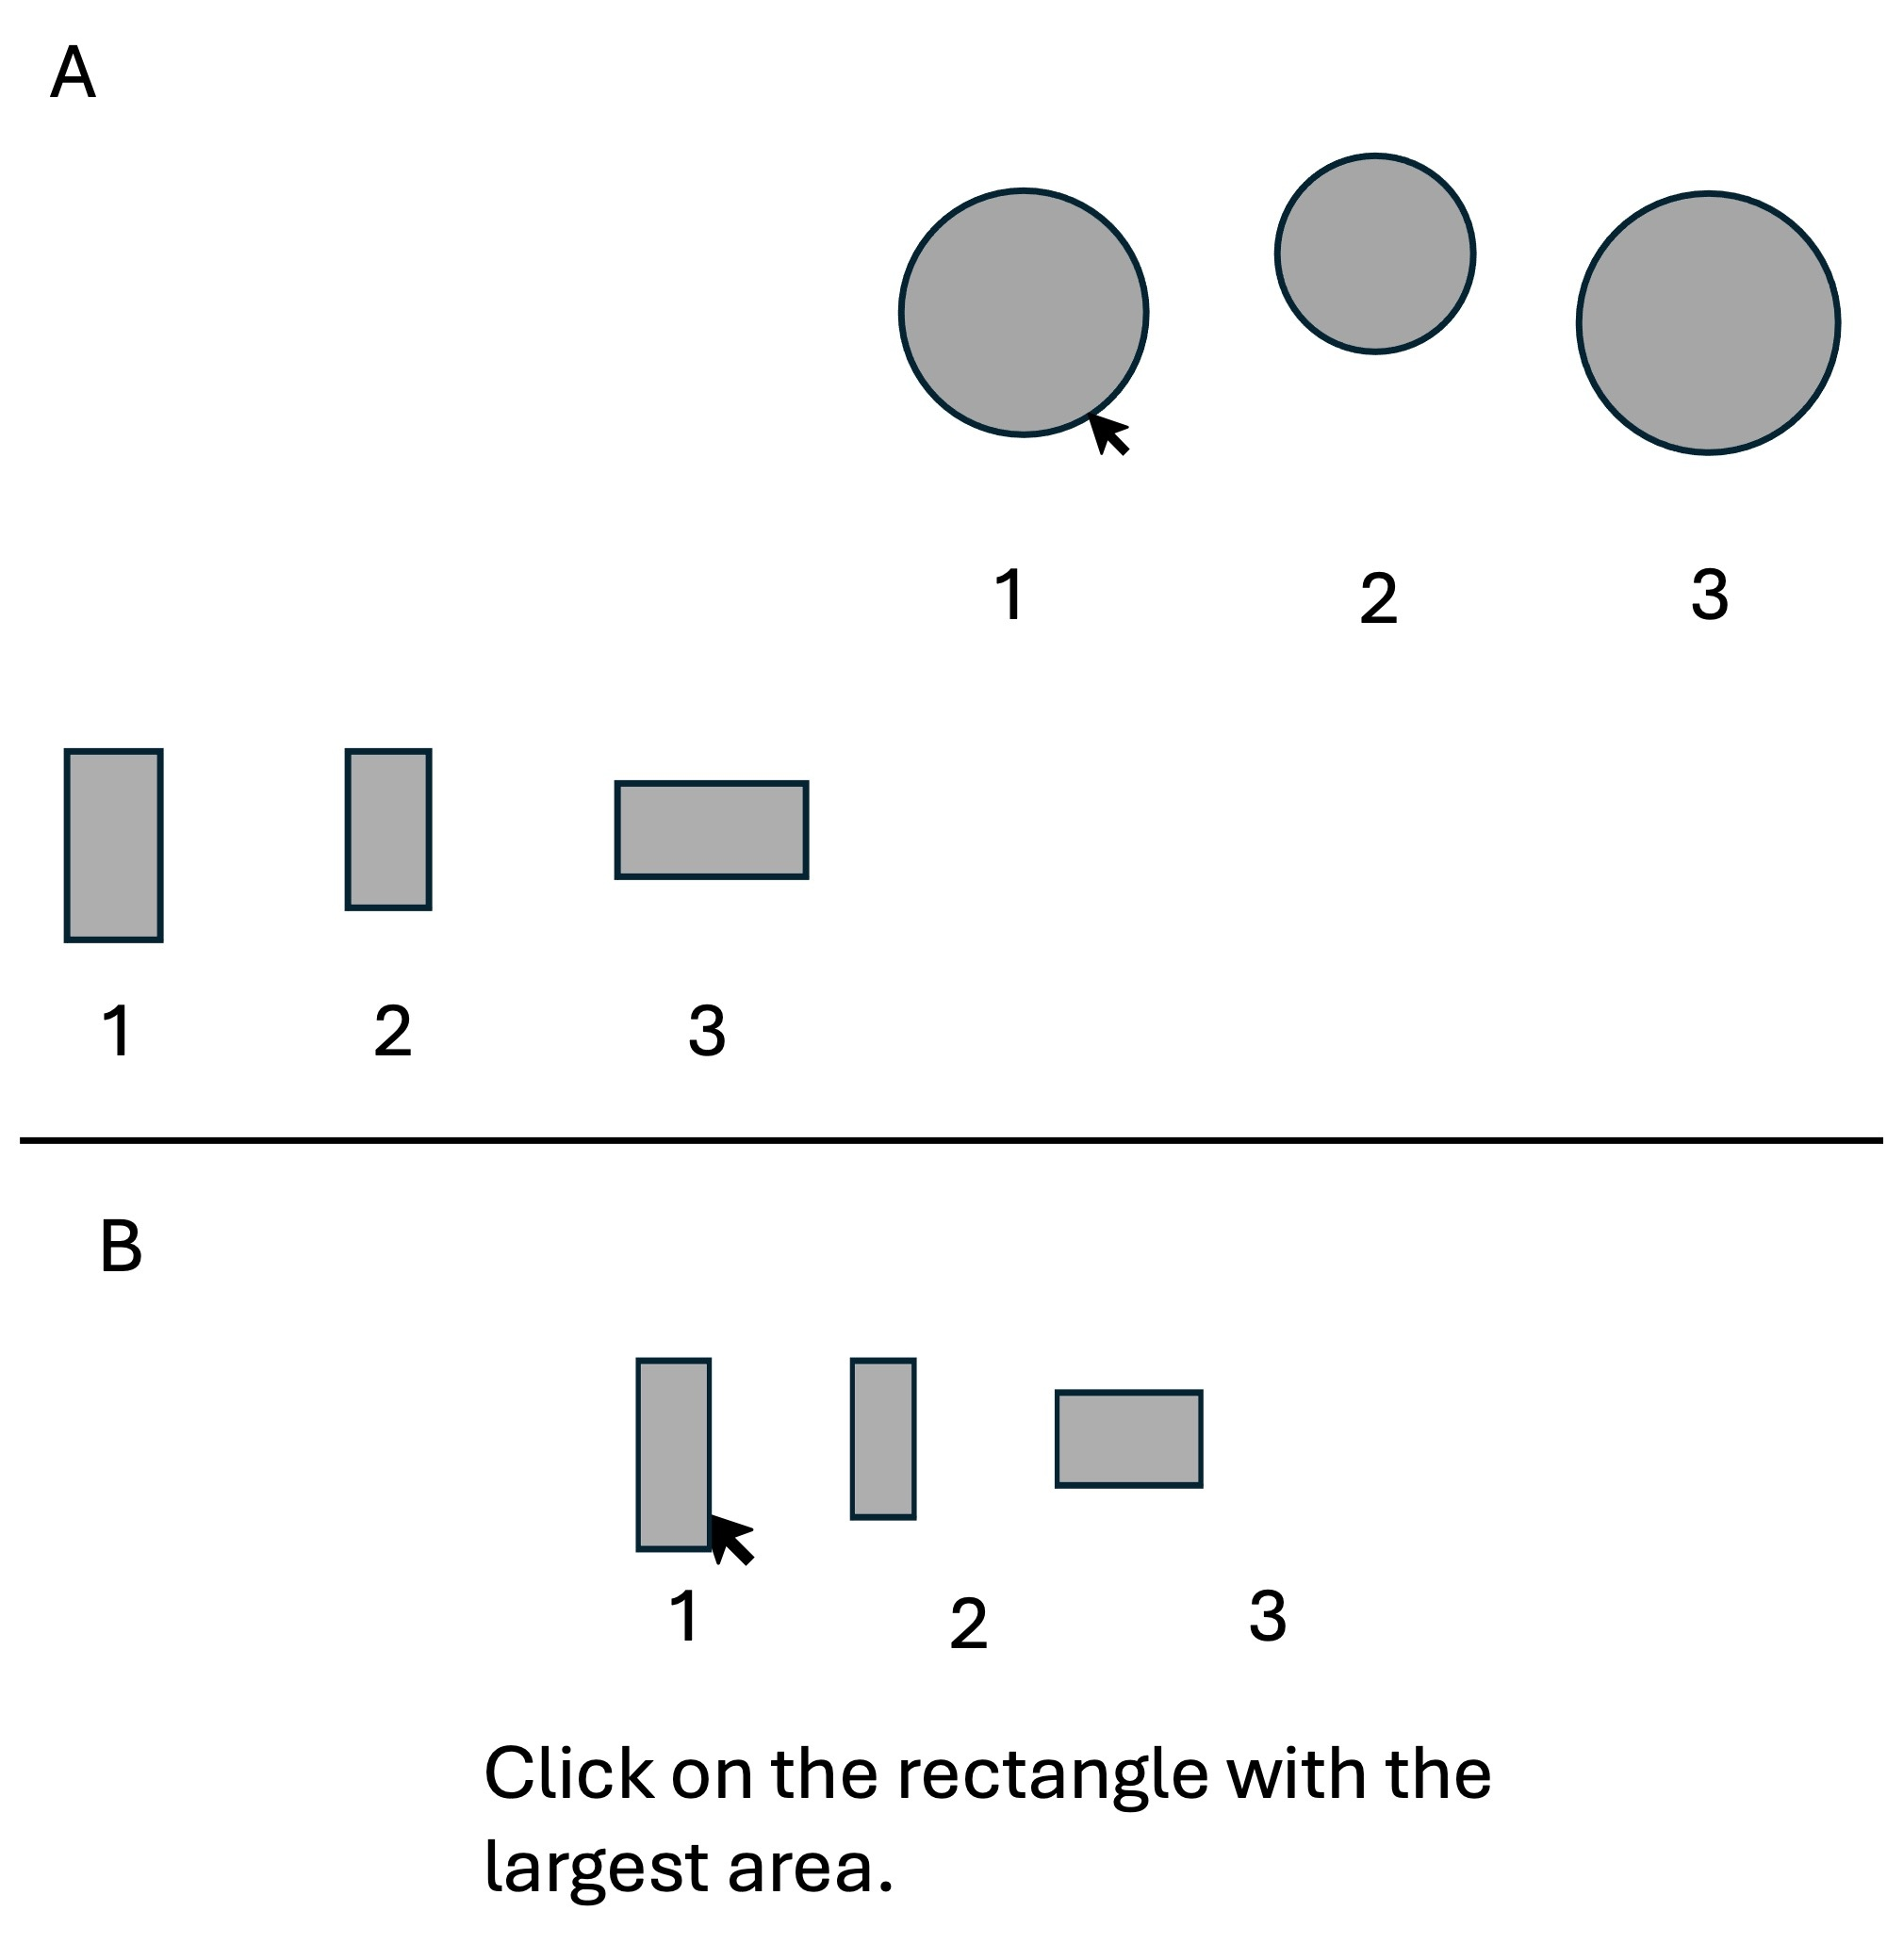
\includegraphics[width=\linewidth]{figures/circle_exp_display.jpg}
   \caption{Example trials from Experiment 2. A: Circle adjustment phase. B: Choice phase. This an example from the horizontal display condition.}
   \label{fig:circle_exp_display}
\end{figure}

\subsection{Results}
\subsubsection{Data Processing}
Given the difficulty of the circle adjustment task, the data required processing to ensure that outlier trials and participants did not influence estimates of $\mathbf{\Omega}$.

First, I removed $10$ participants who did not give correct responses on $75\%$ ($6/8)$ of the catch trials from the circle phase. To respond correctly, participants needed to estimate the largest rectangle to be the as larger than the other two rectangles in the trial. This left a total of 443 participants.

Next, from the remaining participants, I first natural log-transformed all responses. I then dropped all trials where at least one circle was not adjusted (i.e., at least one circle was left at the starting size).

I then removed outlier participants using the following procedure:

I fit a linear regression to each individual participants' data, regressing each log circle area on each corresponding log rectangle area. I then computed an $R^2$ for each participant. I then removed all participants whose $R^2$ fell below the $5\%$ quantile for all $R^2$s, which in this case was $.3975$. This removed $23$ subjects, leaving $N=420$ participants, $213 $in the triangle display condition and $207$ in the horizontal display condition. Of the remaining participants, $R^2$ values were high ($M=.67,SD=.12$), indicating they could generally perform the task.

From the $420$ partipants whose data I analyzed, I removed outlier trials from the critical trial data. I did so to ensure that any outliers do not influence estimates of $\rho_{TD}$, $\rho_{TC}$, or $\rho_{CD}$. I z-transformed all log circle areas within each participant and diagonal. I remove all critical trials where at least one z-score had an absolute value above $3.5$, dropping a total of $102$ trials. I dropped $0$, $1$, $2$, and $4$ critical trials from $339$, $62$, $18$, and $1$ participants, respectively. 

After all circle phase data processing, I were left with $20371$ data points in the triangle display condition and $19809$ data points in the horizontal display condition, where a data point is a vector of participant's estimated target, competitor, and decoy areas. Note that it is crucial to collect a large amount of data here, as performing Bayesian inference on correlation matrices is not straightforward and is prone to underestimation if data is limited \parencite{martin2021,merkle2023opaque}. 

For the choice phase, I only retained participants whose data I retained in the circle phase. All choice trials with RTs $<100\text{ms}$ or $>10,000\text{ms}$ were removed from analysis.

\subsubsection{Circle Phase Results}
Before modeling the data, I first assessed performance on the critical trials. While in an absolute sense, excellent performance is quite difficult to achieve, good relative performance is necessary for any modeling analysis. I computed the mean difference between actual log area and estimated log area for each subject, stimulus pair (i.e., target-competitor, target-decoy, competitor-decoy), and actual difference. I plot these via a set of boxplots in Figure~\ref{fig:circle_boxplots}. Although participants vary considerably in their judgments, I find that on average, participants' adjusted circle areas increase with the absolute size of rectangles. 


\begin{figure}
   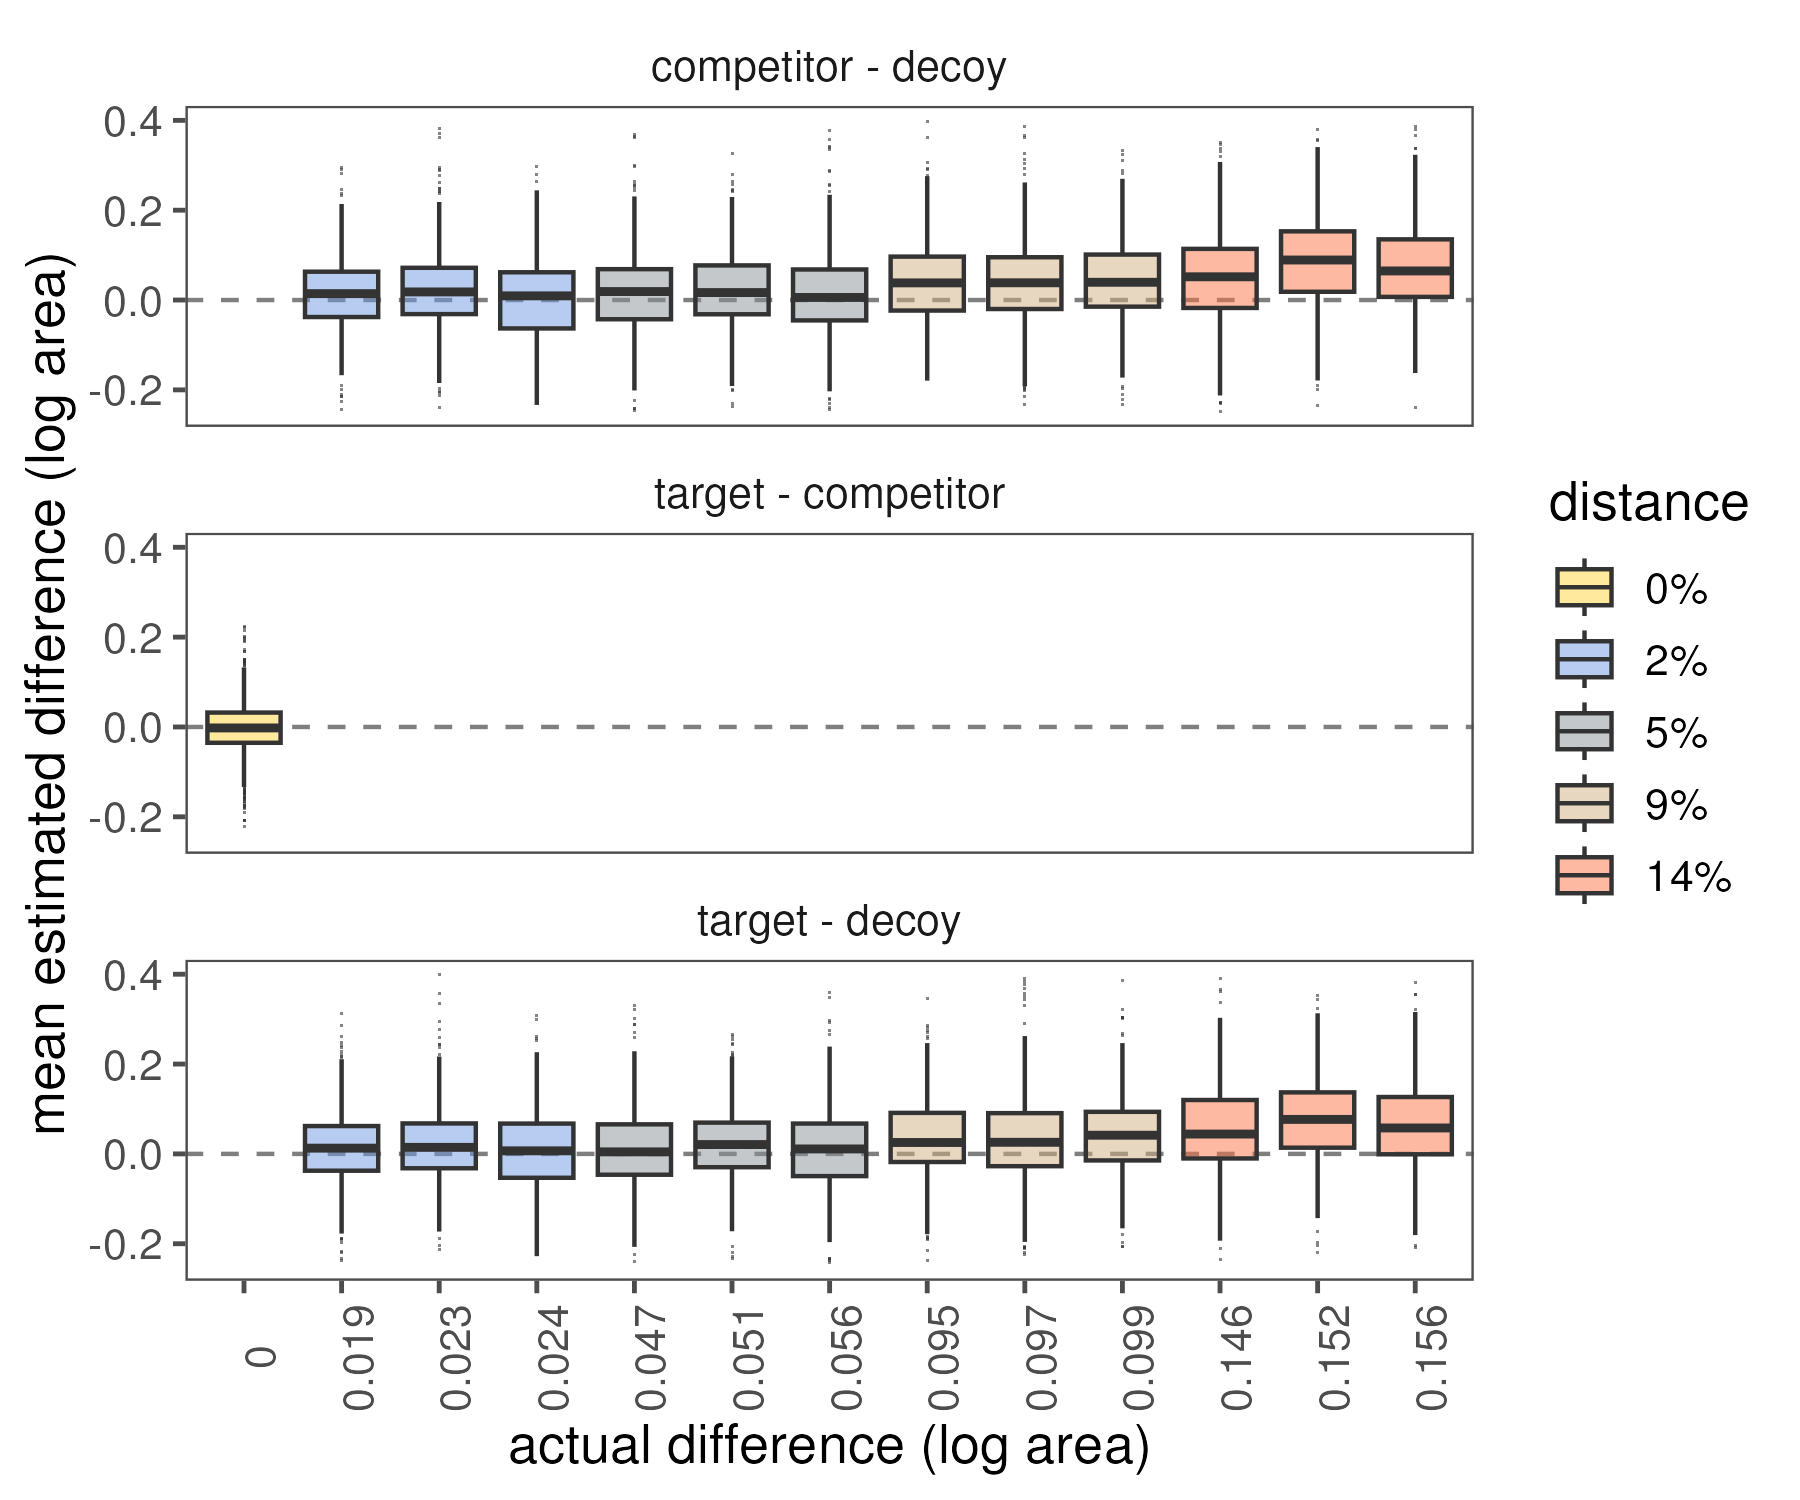
\includegraphics[width=\textwidth]{figures/circleAreaPhase_boxplot_meanlogdiffs_no_outliers.jpeg}
   \caption{Experiment 2 boxplots of subject-level mean error in log-transformed area estimations, split by stimulus pair, TDD, and absolute discrepancy in rectangle area. Note that because the target and competitor rectangles always had equal areas, the true difference is always 0.}
   \label{fig:circle_boxplots}
\end{figure}

I next present scatterplots of all pairwise circle areas from each trial, see Figure~\ref{fig:raw_cors}. I present these to be transparent about the raw data and to illustrate the necessity of a statistical model to understand these correlations. 

\begin{figure}
   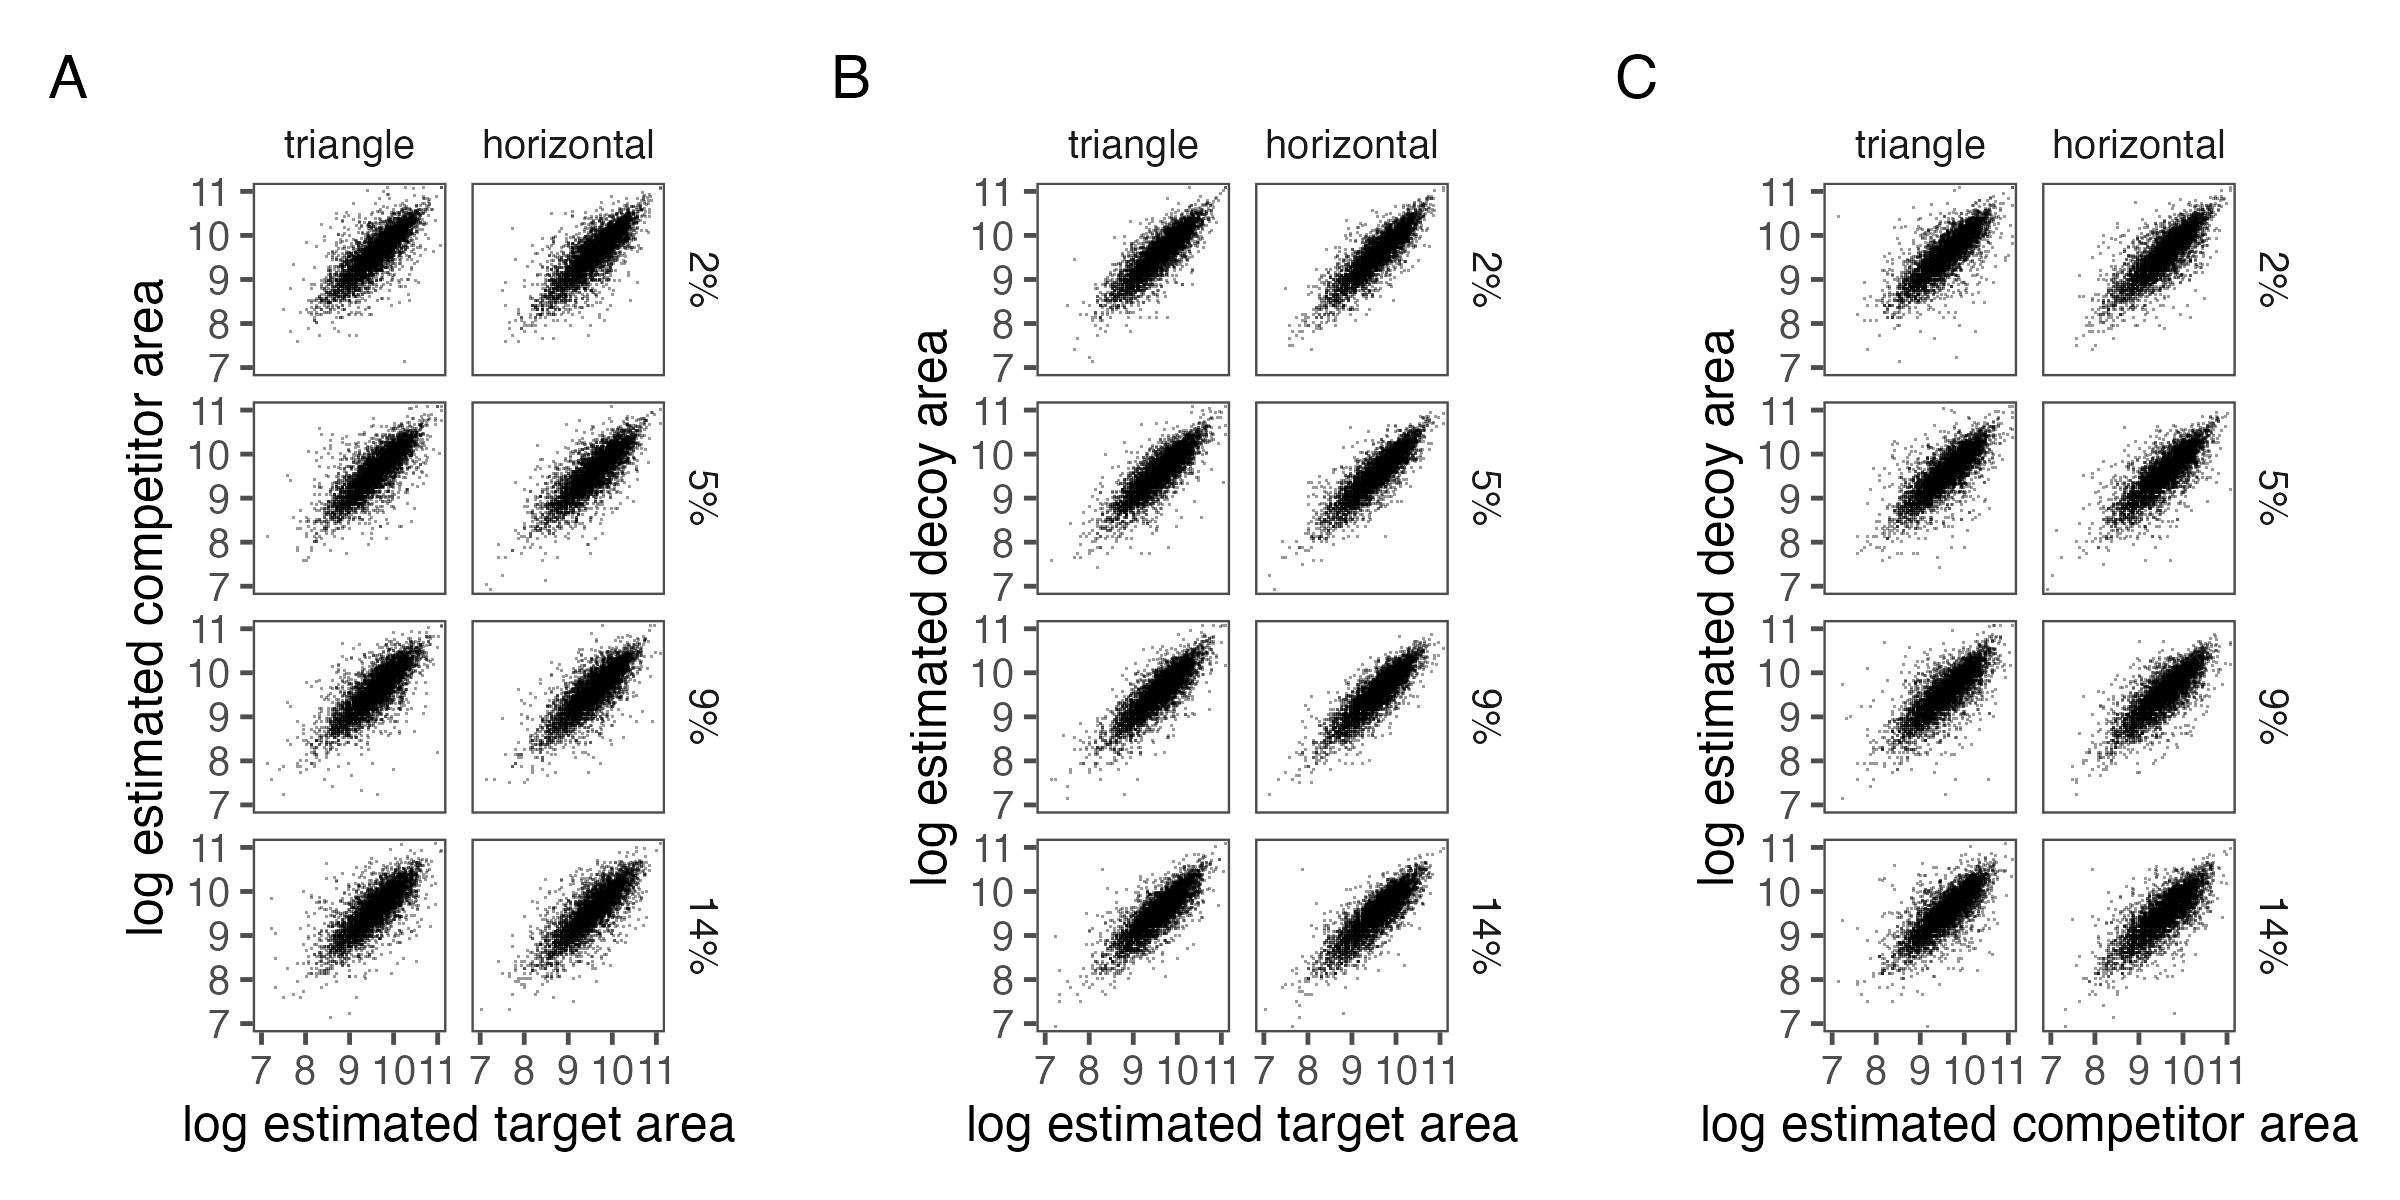
\includegraphics[width=\textwidth]{figures/circleAreaPhase_cor_plot_all_no_outliers.jpg}
   \caption{Scatterplots of target-competitor (A), target-decoy (B), and competitor-decoy (C) log estimated areas, split by display condition and TDD.}
   \label{fig:raw_cors}
\end{figure}

Computing raw correlations, without accounting for subject-level differences, will grossly inflate the size of these correlations. Moreover, any differences between, say, $\rho_{TD}$ and $\rho_{CD}$ are bound to be small. Additionally, performing inferences about the differences between correlations requires Bayesian inference. 

I used Bayesian hierarchical modeling to estimate the parameters of the perceptual model outlined earlier in this chapter. Parameters $\boldsymbol{\mu}$ and $\boldsymbol{\Sigma}$ represent the mean and variance-covariance matrix of a multivariate normal distribution on the perceived areas across trials. 

I assume that, for participant $i$, on each critical trial $j$, the vector of perceived target, competitor, and decoy areas $\mathbf{X_{ij}}$ is sampled from a multivariate normal distribution with mean vector $\boldsymbol{\mu_{ij}}$ and variance-covariance matrix $\boldsymbol{\Sigma}$. 

As discussed in the Introduction, I decompose $\boldsymbol{\Sigma}$ into the  matrix $S\boldsymbol{\Omega}S$, where the diagonal elements of $S$ are population standard deviations and the off diagonal elements are $0$. $\boldsymbol{\Omega}$ is 3 x 3 correlation matrix. Note that there are no participant-level effects in the estimates of $\boldsymbol{\Omega}$.

I focus on the estimates of $\boldsymbol{\mu}$ and $\boldsymbol{\Omega}$ in the main text and discuss the details of the estimation procedure, along with $S$ estimates, in the Appendix. 

I show mean estimates of $\boldsymbol{\mu}$ (averaged across participants) in Figure~\ref{fig:e2mu} and show estimates of $\boldsymbol{\Omega}$ in Figure~\ref{fig:e2_omega}. As predictd, in both conditions, $\rho_{TD}$ is larger than both $\rho_{CD}$ and $\rho_{TC}$, while $\rho_{CD}$ and $\rho_{TC}$ do not differ from each other. Interestingly, all $\rho$ parameters from the horizontal condition are larger than the corresponding parameters from the triangle condition. These inferences should, however, be taken cautiously given that I fit the model separately to each condition.

\begin{figure}
   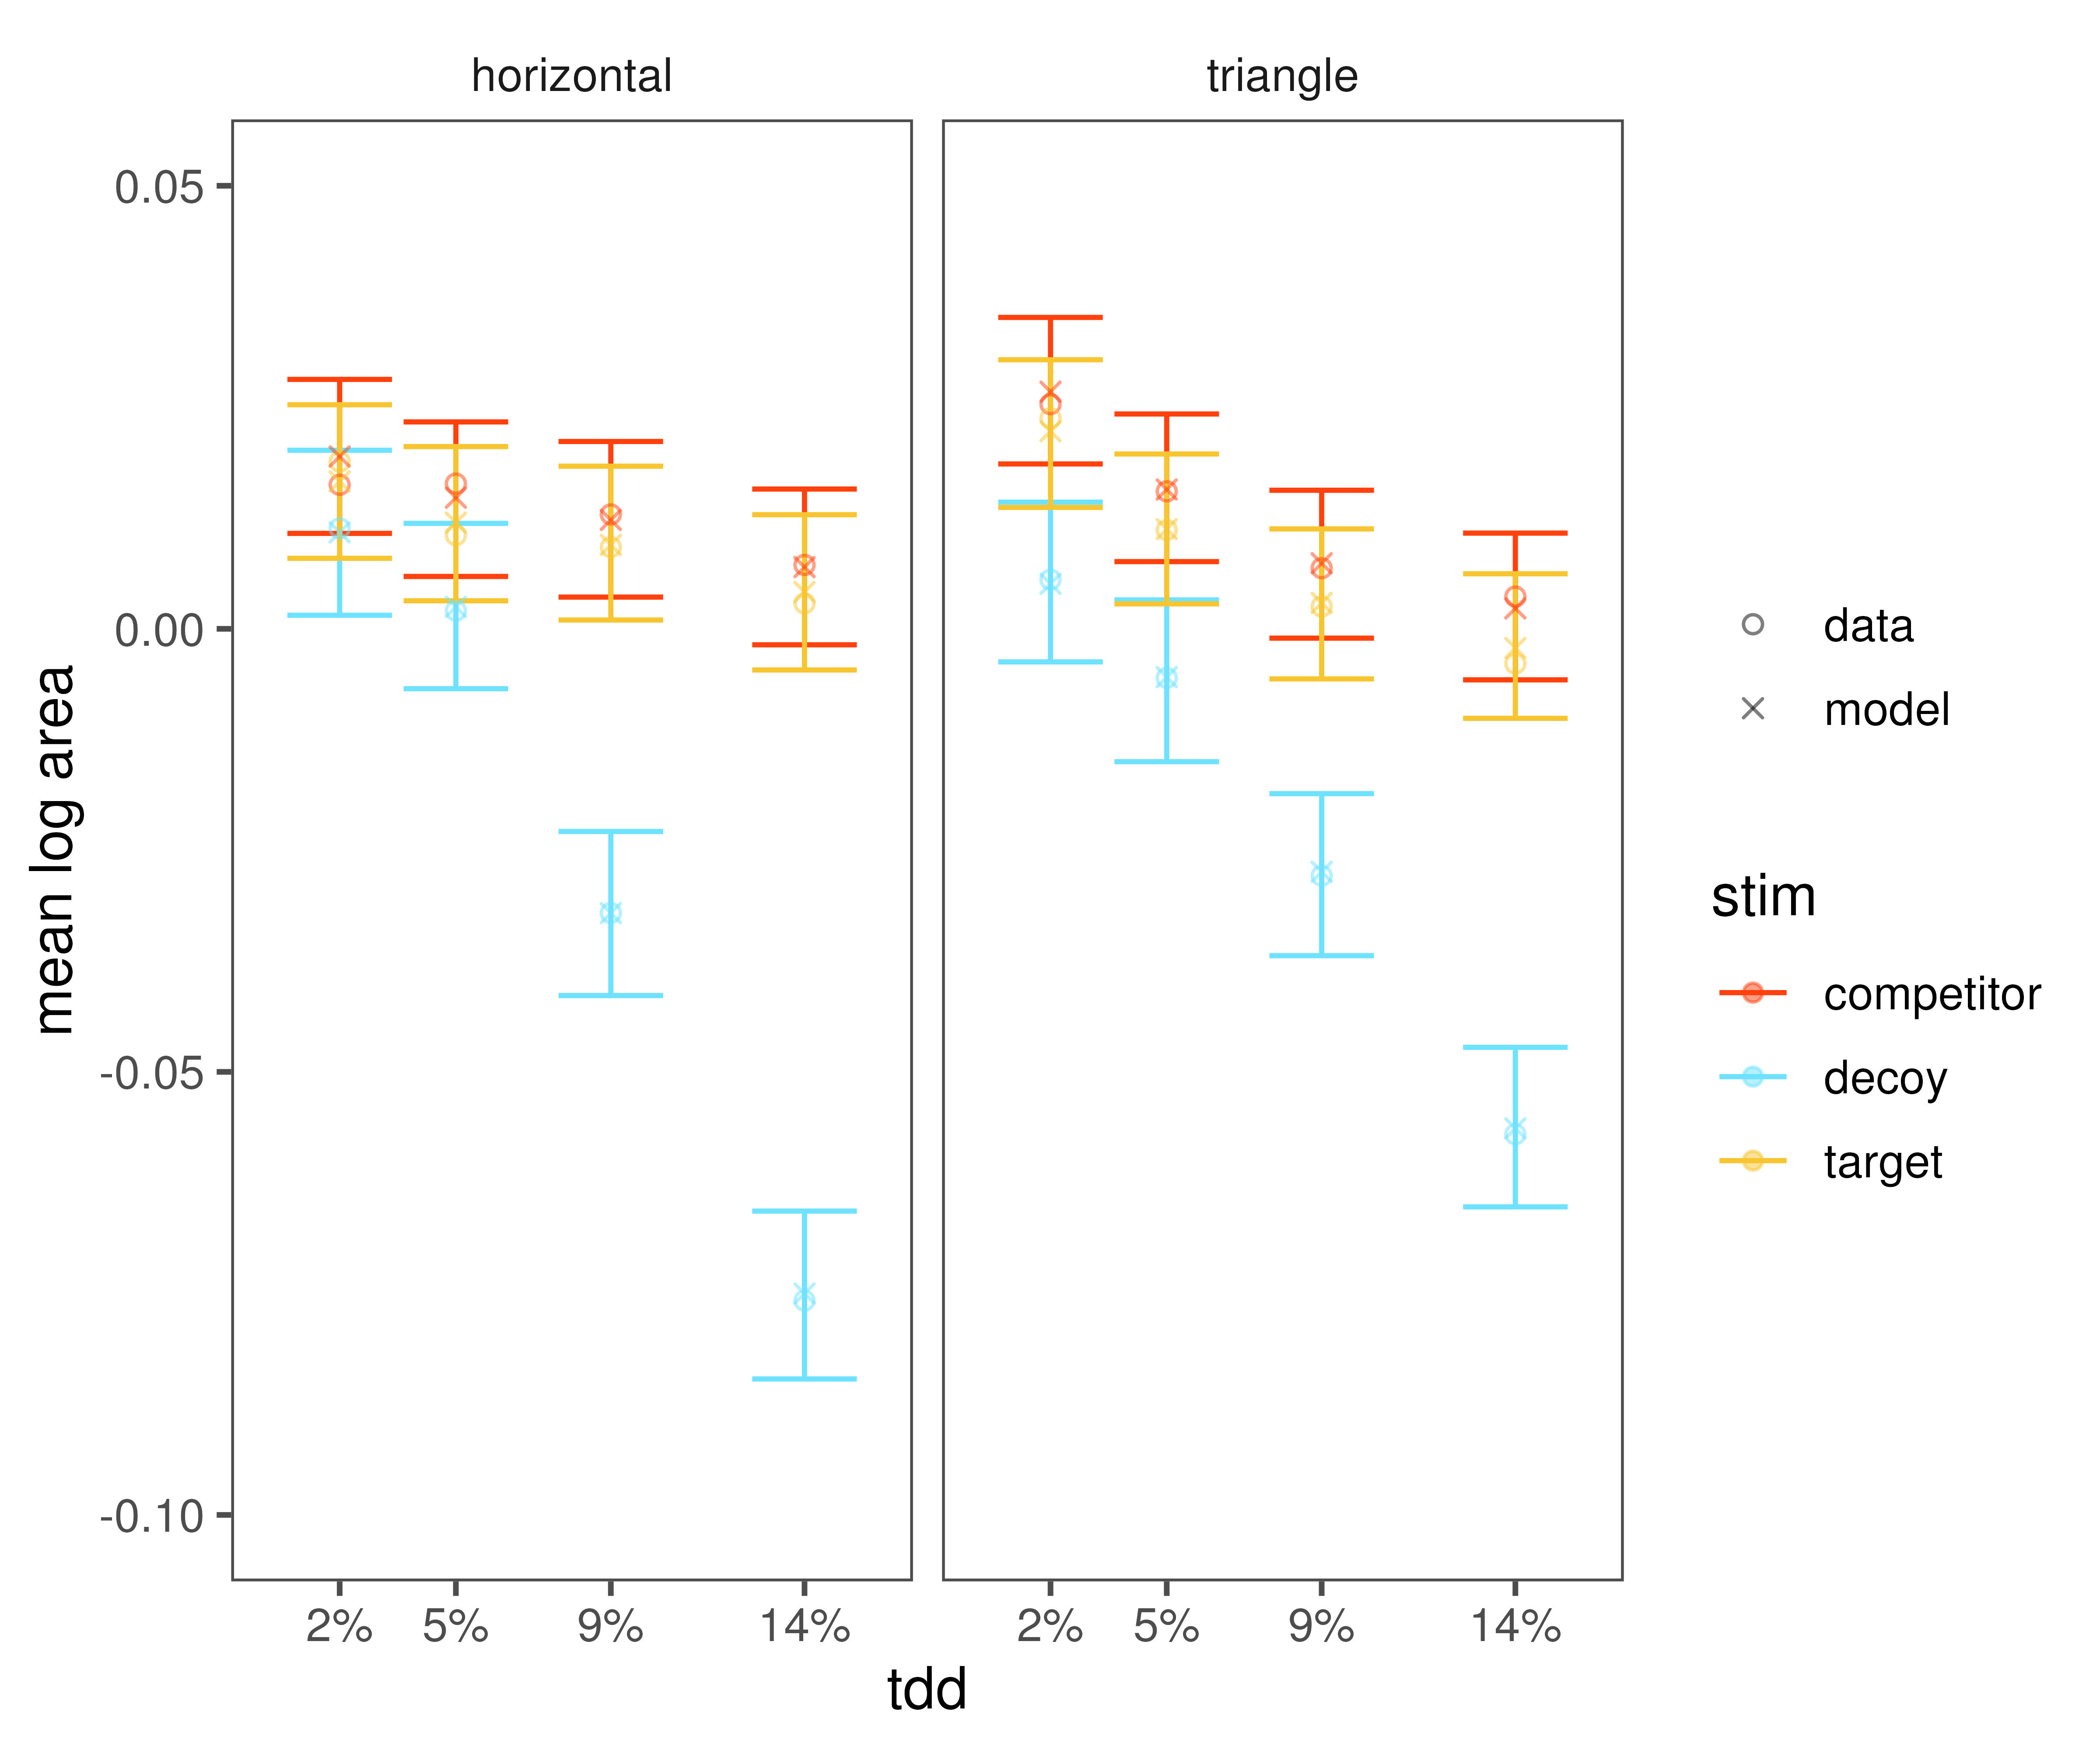
\includegraphics[width=100mm]{figures/bayes_circle_area_mu_sigma_constant_comp_effect_model_v_data_collapsed.jpeg}
   \caption{Experiment 2 $\boldsymbol{\mu}$ estimates. Model values are means, and the error bars are $95\%$ HDIs.}
   \label{fig:e2mu}
\end{figure}

\begin{figure}
   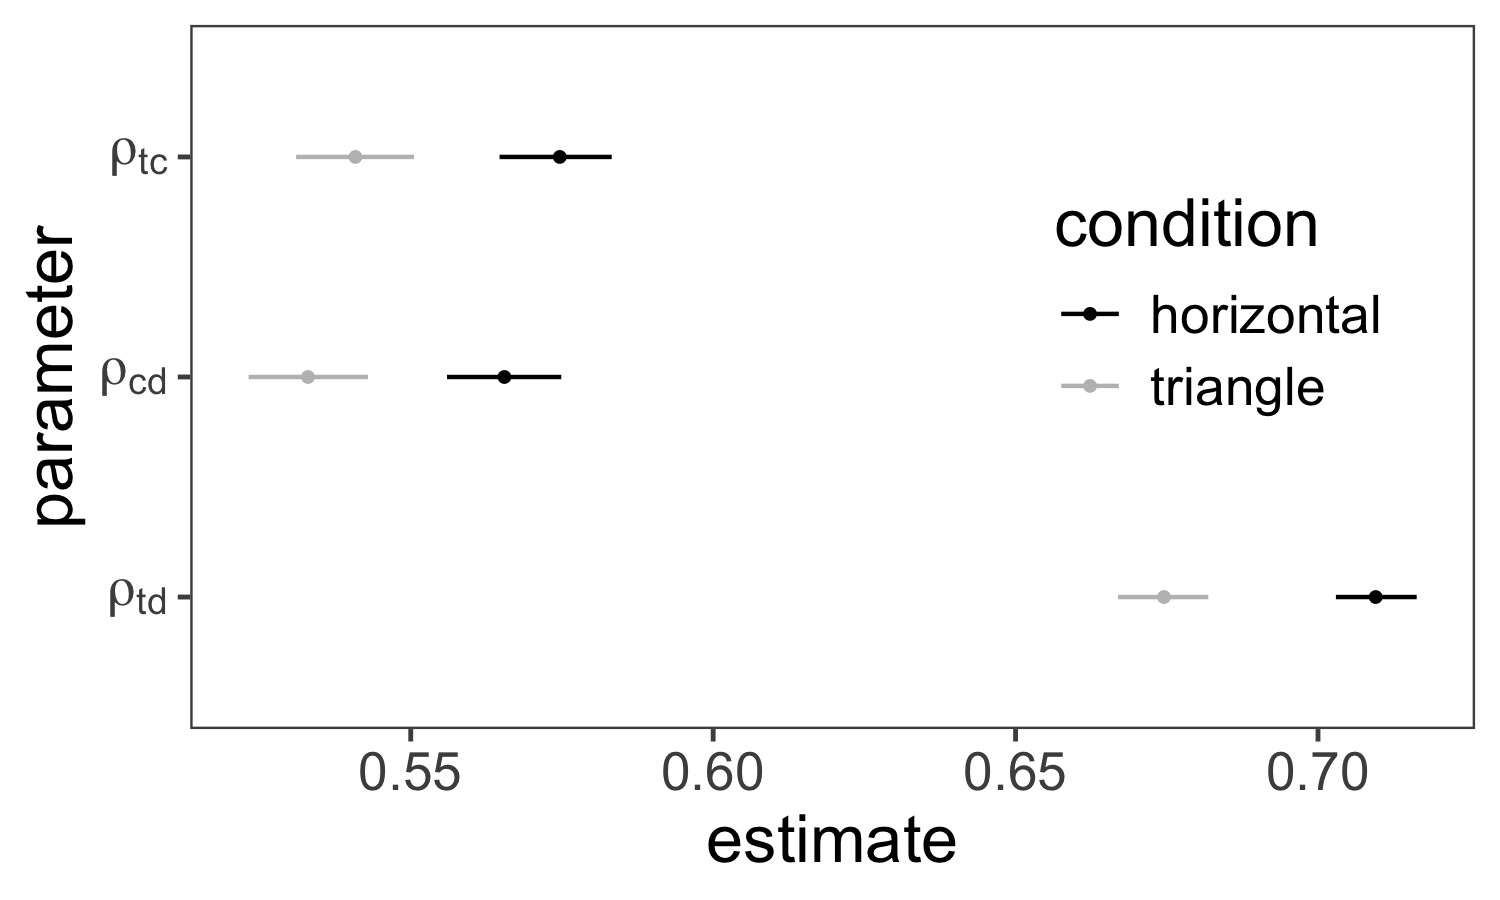
\includegraphics[width=100mm]{figures/bayes_circle_area_sigma_constant_comp_effect_omega_plot.jpeg}
   \caption{Experiment 2 posterior estimates of $\boldsymbol{\Omega}$ off-diagonal parameters across display conditions. Lines show $95\%$ HDIs.  Dots indicate means.}
   \label{fig:e2_omega}
\end{figure}

\subsubsection{Choice Results}

I present mean choice proportions across display conditions and TDD in Figure~\ref{fig:e2_choiceprops}. 

I replicated the qualitative results of \textcite{spektorWhenGoodLooks2018b}. At low levels of TDD, I find a repulsion effect in both display conditions, where participants reliably choose the competitor more than the target. At higher levels of TDD, I either find a small repulsion effect, where $P(C)>P(T)$ (triangle condition) or an attraction effect, where $P(T)>P(C)$ (horizontal condition). See the Appendix for inferential statistics that support these conclusions.

\begin{figure}
   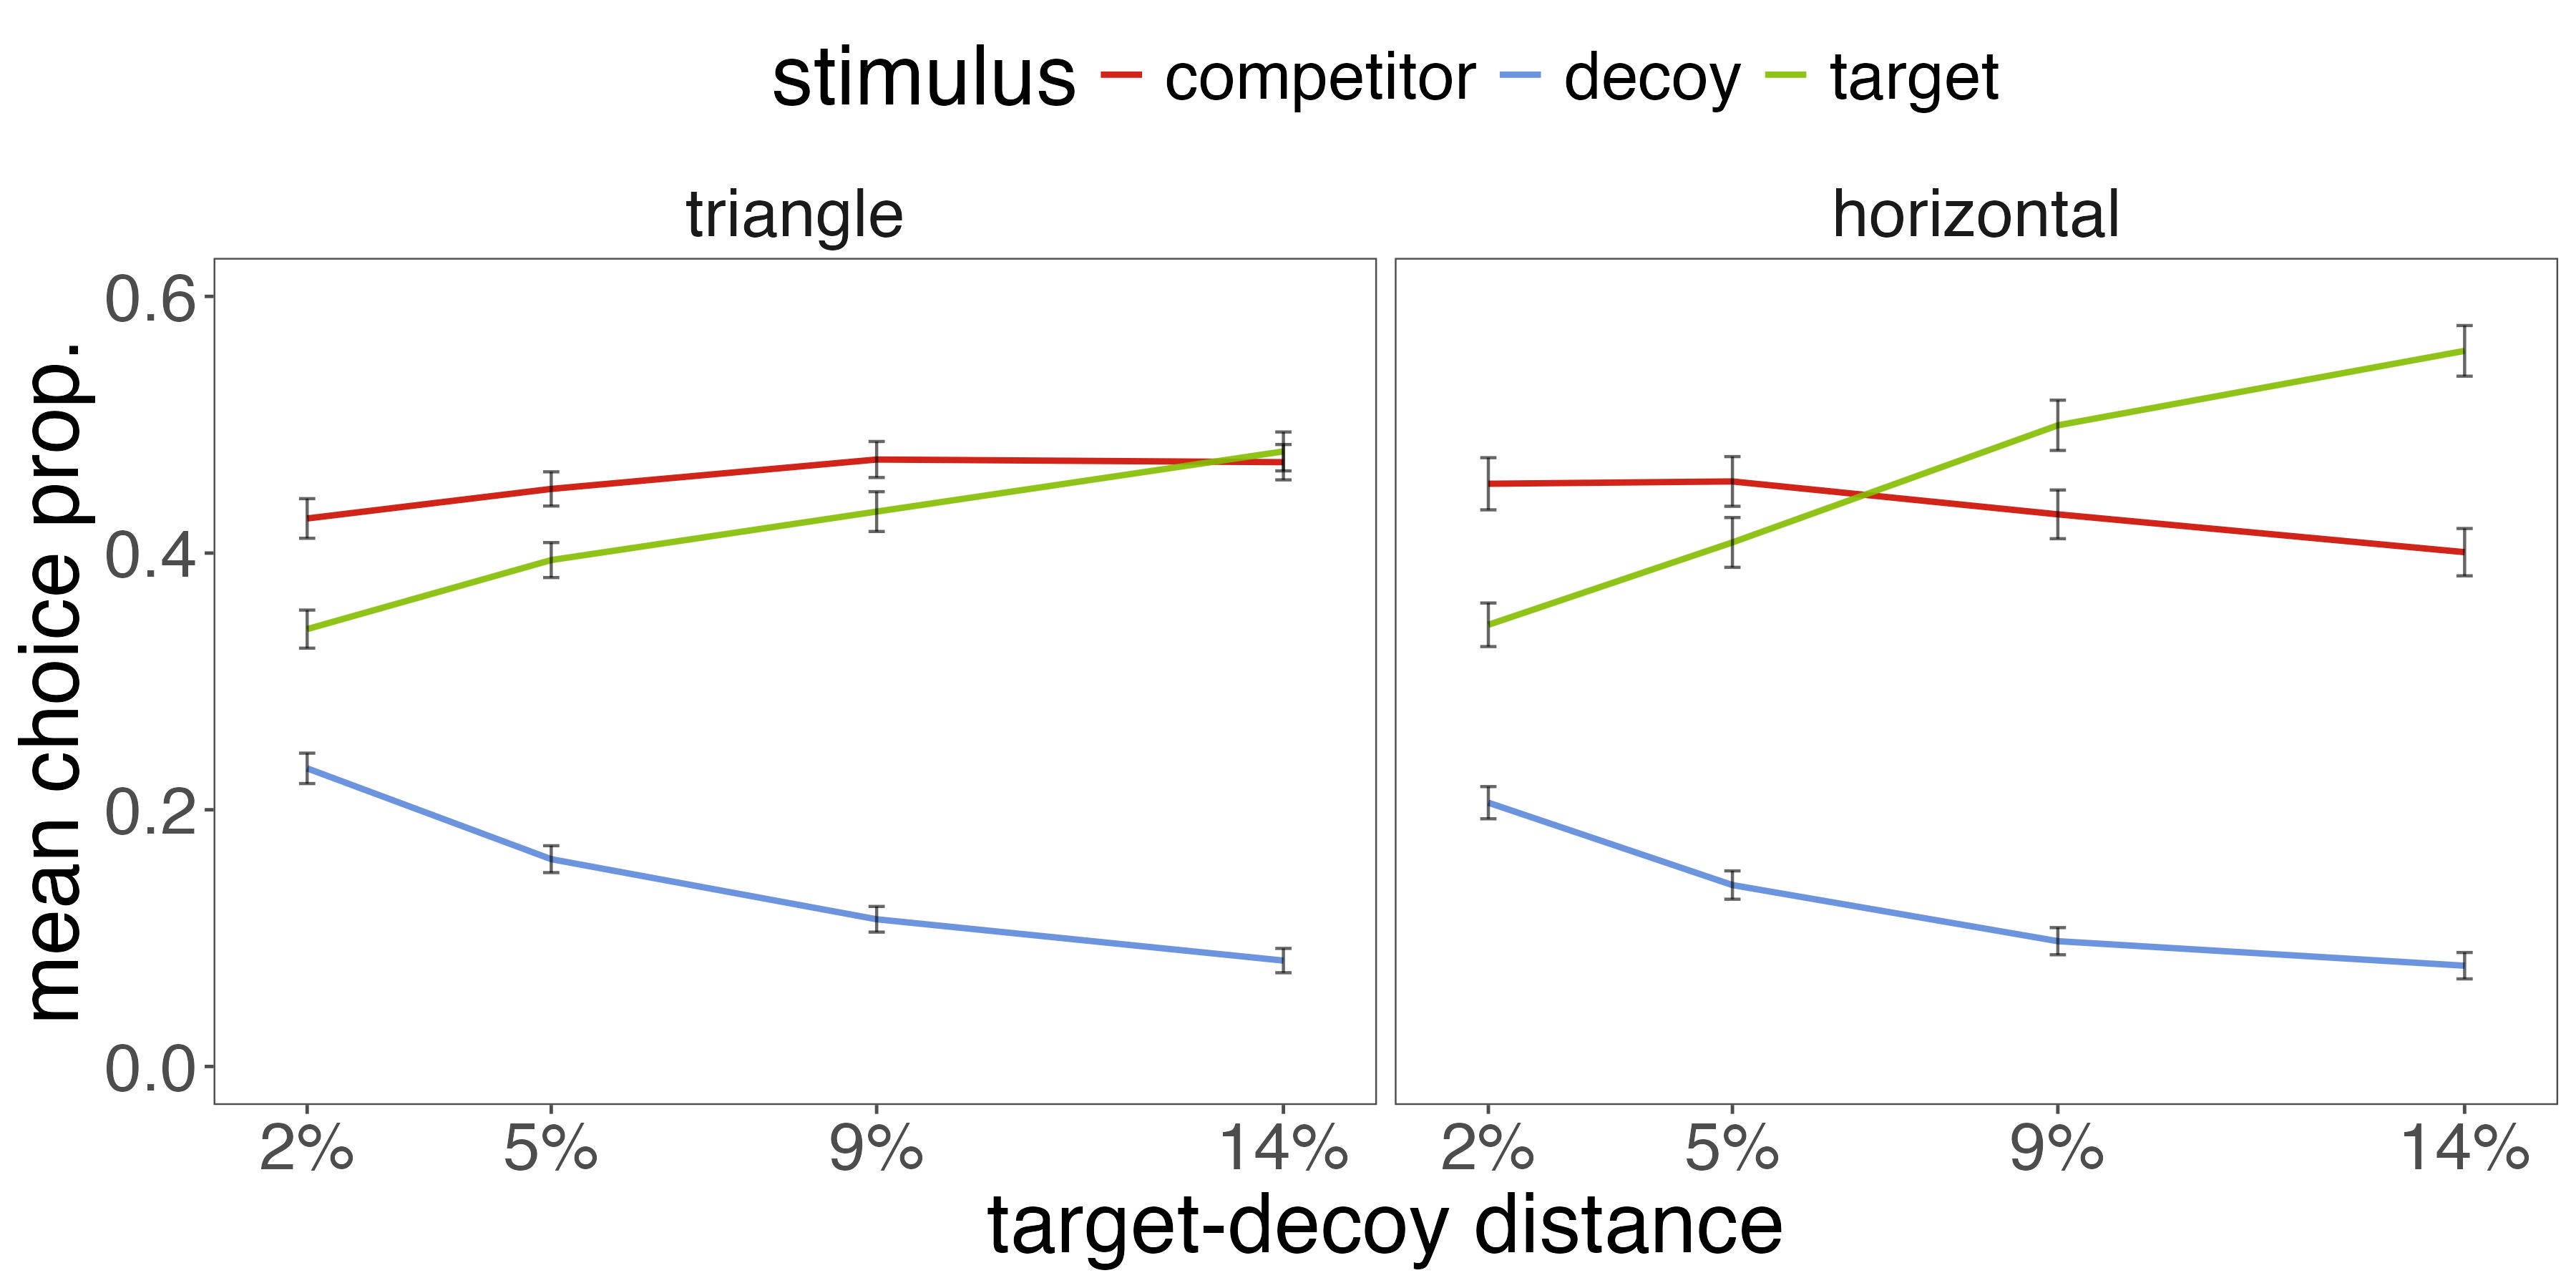
\includegraphics[width=\textwidth]{figures/choicePhase_att_trials_mean_choice_props_collapsed.jpg}
   \caption{Experiment 2 mean choice proportions for target, competitor, and decoy options, by TDD and display condition. Error bars are $95\%$ CIs on the means.}
   \label{fig:e2_choiceprops}
\end{figure}

I also present the mean choice proportions for the current experiment plotted against mean target-decoy discriminability from Experiment 2 in Figure~\ref{fig:e2_choice_compare_to_2afc}. These results strongly indicate that the attraction and repulsion effects are related to the perceptual relationship between target and decoy. 

Furthermore, when comparing across display conditions, the results show that the point at which the repulsion effect becomes a null effect is strongly related to discriminability. Note that this "crossover" point occurs at lower TDD levels for the horizontal condition. In other words, the ease of inter-stimulus comparability in the horizontal condition, which facilitates better discriminability in the 2afc discrimination task, also requires less discrepancy between target and decoy size in order for the attraction effect to emerge in the ternary choice task.

\begin{figure}
   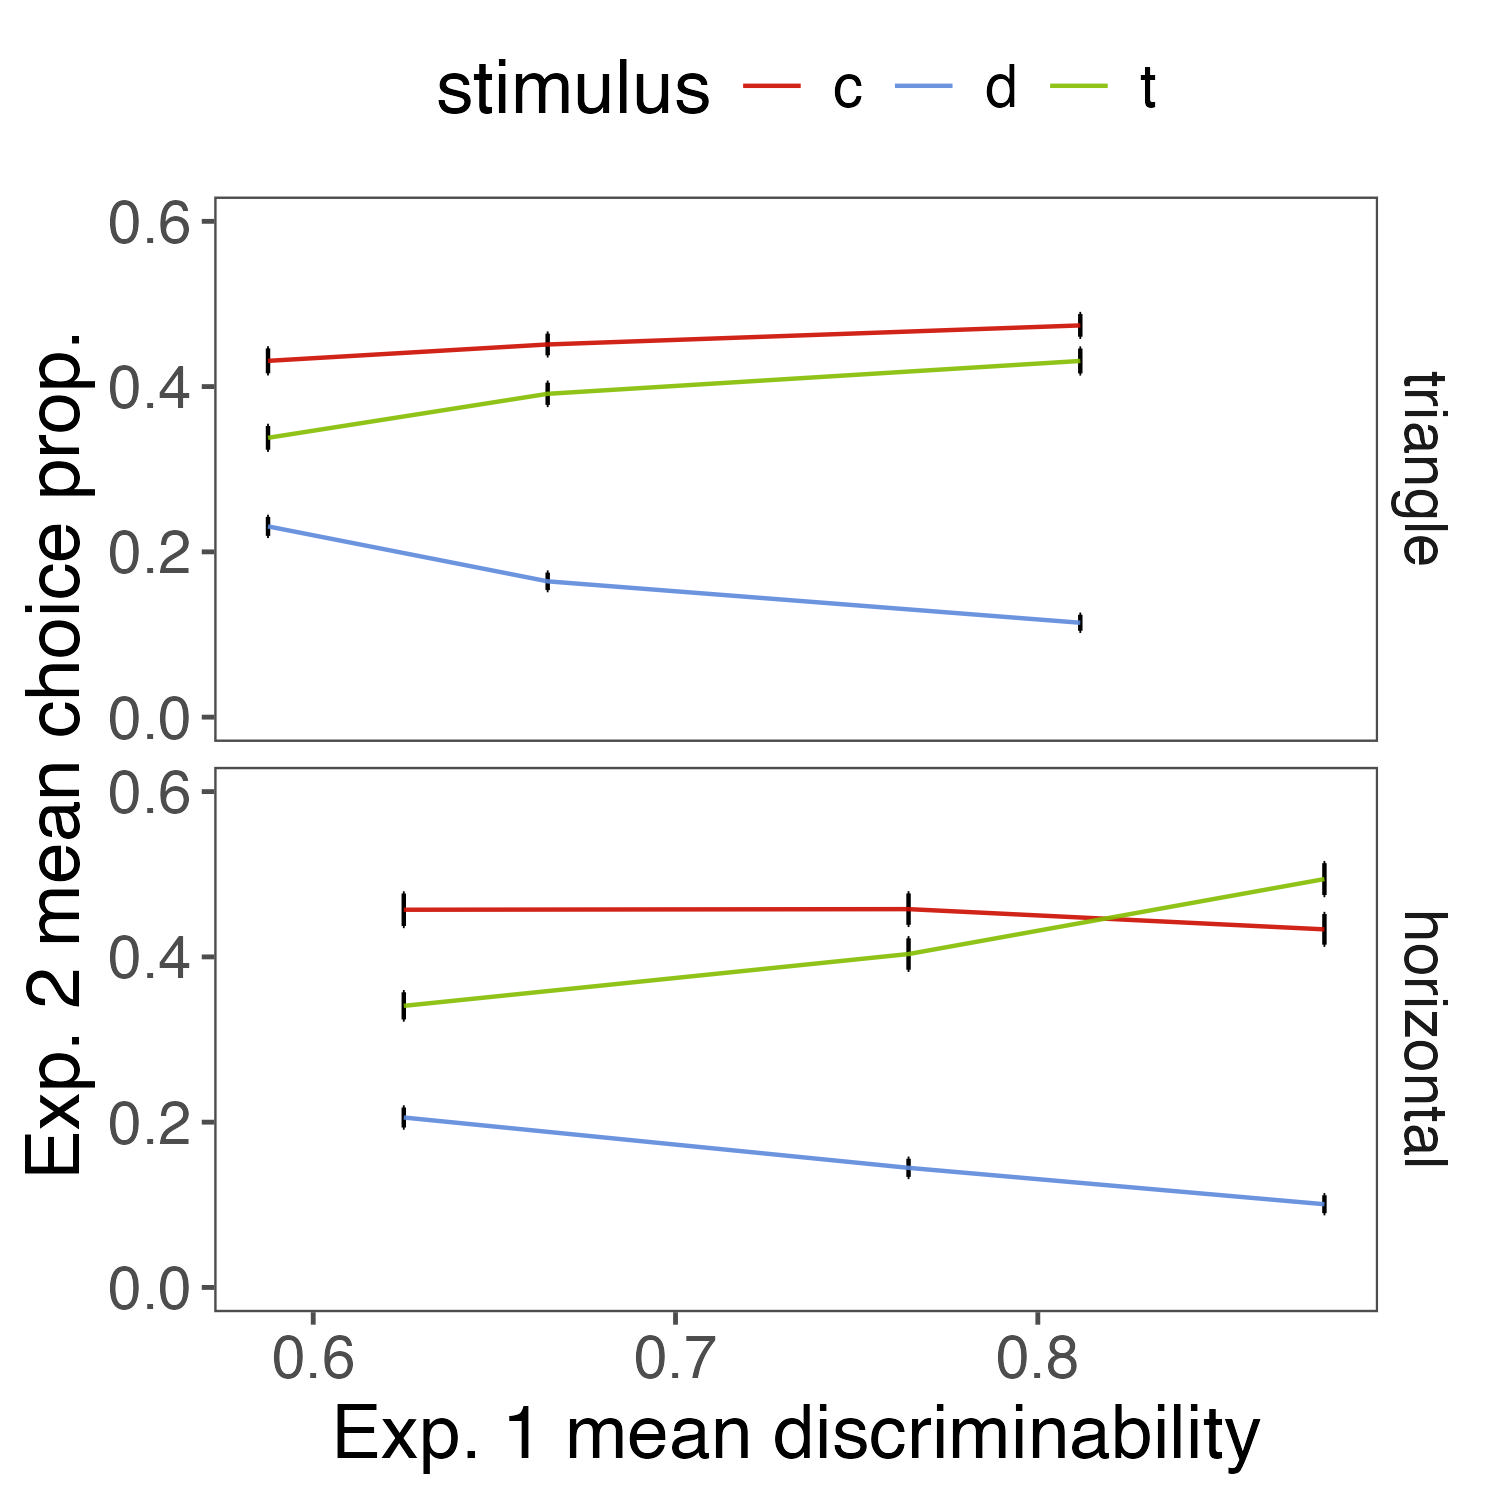
\includegraphics[width=\textwidth]{figures/choicePhase_att_trials_compare_to_2afc_collapsed.jpeg}
   \caption{Mean target, competitor, and decoy choice proportions (y axis) for each TDD level in Experiment 2, plotted against mean target-decoy discriminability for each TDD level from Experiment 1. The x axis error bars are $95\%$ HDIs on the mean, computed via the Bayesian hierarchical logistic regression from Experiment 1, and the y axis error bars are $95\%$ CIs on the mean.}
   \label{fig:e2_choice_compare_to_2afc}
\end{figure}

\subsection{Model Simulations}
After estimating the parameters of the Thurstonian perceptual choice model and analyzing the choice data, I sought to test whether the model can predict the choice data. Though I showed in the introduction that this is possible, it was an open question whether the parameters estimated from actual data would produce qualitatively accurate predictions.

I used the mean estimates of $\boldsymbol{\mu}$ and $\boldsymbol{\Sigma}$ to generate predictions at each level of TDD in both display conditions. I present the predicted mean choice proportions in Figure~\ref{fig:e2_model_preds}. 

\begin{figure}
   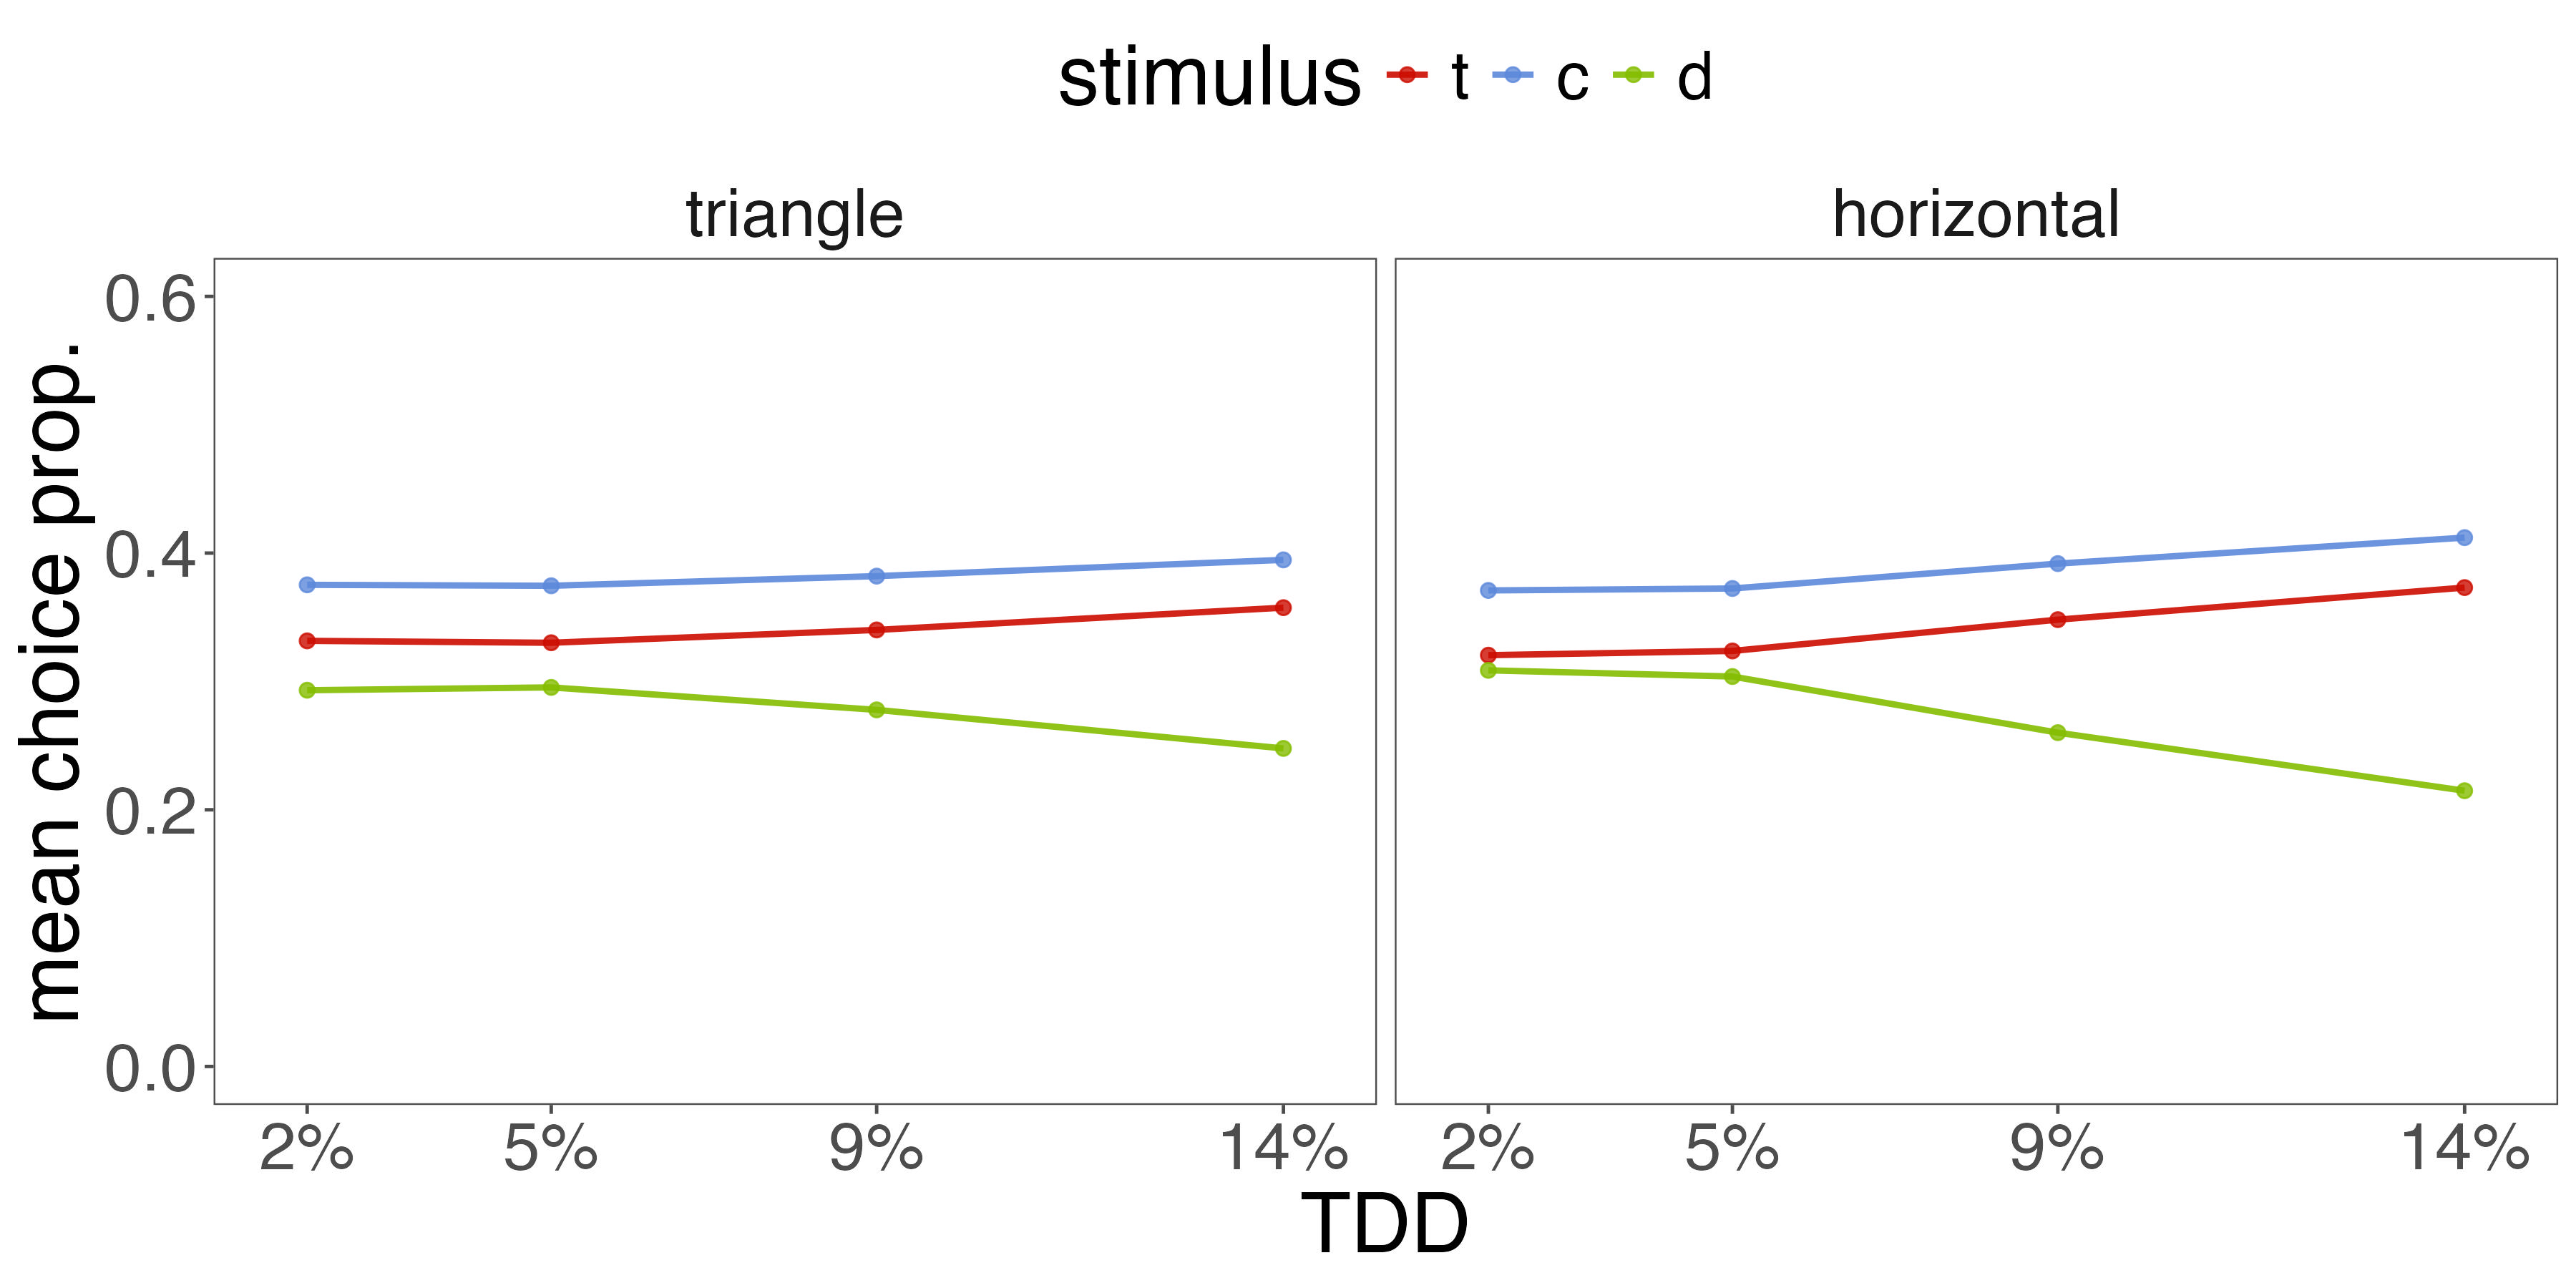
\includegraphics[width=\textwidth]{figures/bayes_circle_area_sim_choice_sigma_constant_comp_effect.jpeg}
   \caption{Model predictions for the choice data, conditioned on the mean estimated parameters from Experiment 2.}
   \label{fig:e2_model_preds}
\end{figure}

Given the estimated parameters, the model is able to produce a repulsion effect. This aligns with our predictions from the introduction; the repulsion effect, at least in some forms, can be generated by a higher correlation between target and decoy stimuli compared to target-competitor and competitor-decoy pairs.

The model fails in predicting the null effect found at high TDD levels in the triangle condition, and it also fails completely in predicting the attraction effect. This is unsurprising, as to produce the attraction effect the model requires either $\mu_{T}>\mu_{C}$ or $\rho_{CD}>\rho_{TD}$, neither or which were found. The model can produce the repulsion effect from perceptual variability alone, but the attraction effect likely occurs due to higher level decision factors.

\section{Discussion}

The results of Experiments 1 and 2 show that participants are not always able to discriminate the decoy from the target and the competitor, and, that target-decoy perceptions appeared to be correlated. The observed correlations can, when embedded in a Thurstonian perceptual choice model, naturally produce the repulsion effect but not the attraction effect. This result is highly informative for decision-making research, as it shows to what extent the effects reported by \textcite{trueblood2013not} and \textcite{spektorWhenGoodLooks2018b} can be explained by perception alone, and to what extent researchers must invoke higher level decision processes to explain them. 

To understand how the model produces the repulsion effect, consider the following simple simulation. Using a multivariate normal model with parameters $\mu_{T}=\mu_{C}=0$, $\mu_{D}=-0.1$, $\sigma_{T}=\sigma_{C}=\sigma_{D}=\frac{1}{3}$, $\rho_{TC}=\rho_{CD}=.65$, and $\rho_{TD}=.75$ (all comparable values those estimated in Experiment 2), I simulated $1,000,000$ trials of a perceptual choice experiment. On each trial, I computed the \textit{ranking} of all perceived areas; for example, an ranking of "TCD" indicates that the target was perceived as largest, the competitor as second-largest, and the decoy as smallest. The results are plotted in Figure~\ref{fig:sim_orderings}. 

\begin{figure}
   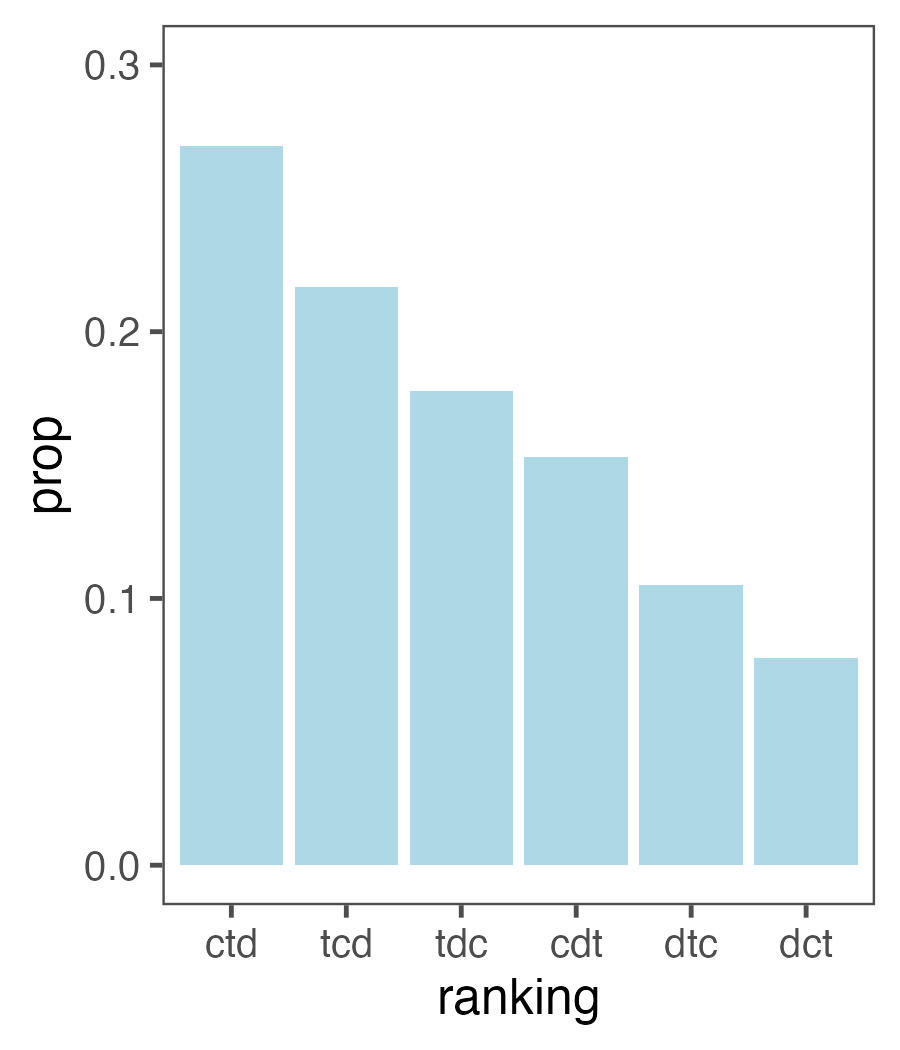
\includegraphics[width=100mm]{figures/sim_mvnorm_rank.jpeg}
   \caption{Model-simulated ranking proportions, in the order of largest to smallest.}
   \label{fig:sim_orderings}
\end{figure}

The results show that $P(CTD)>P(TCD)$, because the target and decoy tend to move together, making it "easier" for the competitor to exceed both options. Furthermore, $P(DTC)>P(DCT)$, because the relatively large $\rho_{TD}$ also allows the decoy to be "pulled up" with the target. These correlations also cause, interestingly enough, $P(TDC)>P(CDT)$. In simple terms, if the decoy is in the middle, it is more likely that the target is the largest than it is that the competitor is largest. Note that if we sum up these orderings we can obtain the marginal choice proportions for $T$, $C$, and $D$ which will show a repulsion effect. 

The correlation between target and decoy perceptions is worth exploring further. Thus far, I have provided a statistical account of these data, but a process account is (one) ultimate goal of cognitive psychology research. I argue that the target and decoy, which are inherently more similar to one another than either is to the competitor, are more likely to be compared to one another. This ease of comparison leads to correlated valuations which in turn affects choice. This account is plausible based both on this research and on prior decision-making research.

\textcite{cataldoComparisonProcessAccount2019b} showed that, in preferential choice, context effects can be reversed or eliminated simply by altering stimulus presentation format. For example, they showed that if participants can easily compare pairs of options (e.g., target and decoy) on each dimension, the attraction effect occurs quite strongly, but without this ease of comparison the attraction effect becomes neglible. \textcite{hasan2025registered}, however, failed to replicate this effect, albeit with different decoys than those of \textcite{cataldoComparisonProcessAccount2019b}. 

\textcite{changWhichCompromiseOption2008} also varied option display, in either a by-alternative format, where option names are listed as columns while attribute values are listed as rows, or a by-attribute format, where option attributes are columns while option names are rows. The former display makes it more difficult to compare options on a single attribute, while the latter makes it easier. They found that listing options by-attribute increased the choice share of the compromise option, relative to a by-alternative display. 

\textcite{hayes2024attribute} manipulated attribute commensurability in a context effects experiment. When two dimensions are commensurable, they vary on a common unit (e.g., user ratings from 0-10), while incommensurable units exist on incomparable units (e.g., RAM and CPU speed in laptops). They found that when dimensions are commensurable, the attraction effect vanishes, while it still exists strongly when dimensions are incommensurable. This suggests that the attraction effect occurs more strongly when the representation of options encourages between-option comparisons on a single attribute.

Furthermore, modern psychological models of context effects often assume an attribute-wise comparison process \parencite{roeMultialternativeDecisionField2001a,trueblood2013not,usherLossAversionInhibition2004a,bhatiaAssociationsAccumulationPreference2013b}. Under this class of models, participants arrive at a decision by comparing pairs of options on a single attribute, where the modeller assumes attribute values are veridical. This assumption is quite reasonable when modeling choices where each attribute is presented separately and discriminability issues are minimal or non-existent. In perceptual choice experiments like those presented here or in \textcite{spektorWhenGoodLooks2018b,trueblood2013not}, these assumptions are likely incorrect. However, the general modeling framework, where inter-stimulus comparison leads to preference, which then leads to choice, is still plausible.

Other researchers have suggested that correlated valuations as a measure of similarity. Multialternative Decision Field Theory (MDFT) \parencite{roeMultialternativeDecisionField2001a} relies on within-trial correlations between similar options to produce the similarity effect, though this mechanism is distinct from the current model, which relies on \textit{across-trial} correlated valuations. 

\textcite{natenzon2019random} implemented a Bayesian probit model, in which participants are assumed to sample from a multivariate normal distribution on each trial, with the correlation between options being related to their similarity in multiattribute space. \textcite{natenzon2019random} also suggests that similarity is related to ease of comparability. They fitted the model to frog mating choice data and showed that not only can the model explain choice reversals (i.e., context effects), but the estimated correlations between pairs of options were greater for options closer in multiattribute space. 

\textcite{kamakura1984predicting} incorporated correlations into a multivariate choice model. According to their model, options in a choice set have utilities which are distributed multivariate normal, with non-zero correlations. The correlations are a decreasing function of distance in attribute space. The researchers fit the model to choice data and show that it can account for the similarity effect in choice (i.e., where two similar options "split" choice shares). Future research should consider whether a model whose correlations are based on directly estimated correlations can predict the similarity effect. 

\textcite{bhui2021rational} showed that target and decoy valuations may be correlated, and they further argued that the repulsion effect is rational given a consumer's belief that the target and decoy come from the same distribution (e.g., two products from the same brand). \textcite{bhui2024context} similarly argued that context effects can be rational given limited information about options in a choice set. 

The results of Experiments 1 and 2 have important methodological implications. \textcite{trueblood2013not} and \textcite{spektorWhenGoodLooks2018b} designed their studies to test the interesting hypothesis that context effects occur even in low-level, perceptual decision-making. They designed experiments similar to other attraction effect experiments, with two equally "valuable" focal options and inferior decoy option which is similar to a focal, target option. They did not fully consider, however, issues in perceptual variability. While acknowledging that participants may occasionally fail to perceive the dominance relationship, they assumed that this would not affect the overall results. They did not consider the possibility, however, that the target-decoy comparability could cause perceptual correlations which manifest themselves in the choie data. \textcite{spektorWhenGoodLooks2018b} even discussed the possibility that their repulsion effect may be a form of the \textit{similarity effect}, where two similar options split choice shares, but they dismissed this hypotheis out of hand because participants chose the target more often than they chose the decoy. I showed in Experiment 2 that despite the fact that $P(T)>P(D)$, the decoy is systematically chosen over the target more than it is chosen over the competitor. 

Researchers have also argued in favor of the "tainting hypothesis" \parencite{simonson2014vices,spektorWhenGoodLooks2018b}, where the inferior decoy "taints" similar options (i.e., the target). On average, participants did generally rate the competitor as larger than the target in Experiment 2. These results were, however, quite small and not always statistically apparent. Moreover, the model does not require this tainting to produce the repulsion effect.

The existence of context effects in perceptual choice is an interesting phenomenon and one that should be studied further. Still, researchers should be careful in assuming that an empirical context effect is generated solely by decision processes whenever the choice environment precludes full stimulus discriminability.

There are some limitations to the current experiment. Due to the large amount of data required to estimate a variance-covariance matrix \parencite{martin2021,merkle2023opaque}, I collapsed across participants when estimating $\boldsymbol{\Omega}$. This may obscure individual differences, an area of increasing concern in context effect research \parencite{liewAppropriacyAveragingStudy2016b,trueblood2015fragile,davis2023illustrated}. Future research should collect enough participant-level data (perhaps by asking participants to return for multiple experimental sessions) to allow participant-level variation in $\boldsymbol{\Omega}$ estimates. It would be of great theoretical interest if individual differences in $\boldsymbol{\Omega}$ could explain individual variation in the attraction and repulsion effects.

As discussed in the Appendix, participants were biased to choose wide rectangles as larger than tall rectangles, but they tended to rate tall rectangles as being larger than wide (at least in the triangle condition). The latter effect is quite small (i.e., smaller than that of the difference between the target and the smallest decoy), but it is nonetheless present in the data. I currently have no strong explanation for this result. \textcite{gronau2023choice} compared participants' ability to perform perceptual discrimination task based on whether they responded via an ordinal rating scale or a choice. The authors concluded that participants relied on the same representation in both cases, but the participants were more sensitive to stimulus-level differences when choice responses were collected. It may be that, in Experiment 2, the relative lack of perceptual sensitivity caused participants to slightly underestimate their reported responses to stimuli they actually \textit{perceived} as larger. This bias reversal may also be idiosyncratic statistical variation, and new samples may fail to show it. It is also not particularly theoretically important. We are mainly interested in target, decoy, and competitor ratings (collapsed across orientation), rather than perception of area \textit{per se}. Nonetheless, this result may be of interest to perceptual (e.g., vision science) researchers.

In the next chapter, I test a prediction of the perceptual model in best-worst choice. I also use these results to test a well-studied theoretical model of the best-worst choice experimental paradigm.
